%% For double-blind review submission, w/o CCS and ACM Reference (max submission space)
\documentclass[sigplan,10pt,review,anonymous]{acmart}\settopmatter{printfolios=true,printccs=false,printacmref=false}
%% For double-blind review submission, w/ CCS and ACM Reference
%\documentclass[sigplan,review,anonymous]{acmart}\settopmatter{printfolios=true}
%% For single-blind review submission, w/o CCS and ACM Reference (max submission space)
%\documentclass[sigplan,review]{acmart}\settopmatter{printfolios=true,printccs=false,printacmref=false}
%% For single-blind review submission, w/ CCS and ACM Reference
%\documentclass[sigplan,review]{acmart}\settopmatter{printfolios=true}
%% For final camera-ready submission, w/ required CCS and ACM Reference
%\documentclass[sigplan]{acmart}\settopmatter{}

\usepackage{fancyvrb}
%% Conference information
%% Supplied to authors by publisher for camera-ready submission;
%% use defaults for review submission.
\acmConference[DLS'19]{Dynamic Languages Symposium}{October 22, 2019}{Athens, Greece}
\acmYear{2019}
\acmISBN{} % \acmISBN{978-x-xxxx-xxxx-x/YY/MM}
\acmDOI{} % \acmDOI{10.1145/nnnnnnn.nnnnnnn}
\startPage{1}

%% Copyright information
%% Supplied to authors (based on authors' rights management selection;
%% see authors.acm.org) by publisher for camera-ready submission;
%% use 'none' for review submission.
\setcopyright{none}
%\setcopyright{acmcopyright}
%\setcopyright{acmlicensed}
%\setcopyright{rightsretained}
%\copyrightyear{2018}           %% If different from \acmYear

%% Bibliography style
\bibliographystyle{ACM-Reference-Format}
%% Citation style
%\citestyle{acmauthoryear}  %% For author/year citations
%\citestyle{acmnumeric}     %% For numeric citations
%\setcitestyle{nosort}      %% With 'acmnumeric', to disable automatic
                            %% sorting of references within a single citation;
                            %% e.g., \cite{Smith99,Carpenter05,Baker12}
                            %% rendered as [14,5,2] rather than [2,5,14].
%\setcitesyle{nocompress}   %% With 'acmnumeric', to disable automatic
                            %% compression of sequential references within a
                            %% single citation;
                            %% e.g., \cite{Baker12,Baker14,Baker16}
                            %% rendered as [2,3,4] rather than [2-4].


%%%%%%%%%%%%%%%%%%%%%%%%%%%%%%%%%%%%%%%%%%%%%%%%%%%%%%%%%%%%%%%%%%%%%%
%% Note: Authors migrating a paper from traditional SIGPLAN
%% proceedings format to PACMPL format must update the
%% '\documentclass' and topmatter commands above; see
%% 'acmart-pacmpl-template.tex'.
%%%%%%%%%%%%%%%%%%%%%%%%%%%%%%%%%%%%%%%%%%%%%%%%%%%%%%%%%%%%%%%%%%%%%%


%% Some recommended packages.
\usepackage{booktabs}   %% For formal tables:
                        %% http://ctan.org/pkg/booktabs
\usepackage{subcaption} %% For complex figures with subfigures/subcaptions
                        %% http://ctan.org/pkg/subcaption
\usepackage{xspace}
\usepackage{multirow}


\newcommand{\todo}[1]{\color{orange}\fbox{\bfseries\sffamily\scriptsize TODO:}{\sf\small$\blacktriangleright$\textit{#1}$\blacktriangleleft$}\color{black}}
\newcommand{\egb}[1]{\color{blue}\fbox{\bfseries\sffamily\scriptsize Elisa:}{\sf\small$\blacktriangleright$\textit{#1}$\blacktriangleleft$}\color{black}}
\newcommand{\eem}[1]{\color{olive}\fbox{\bfseries\sffamily\scriptsize Eliot:}{\sf\small$\blacktriangleright$\textit{#1}$\blacktriangleleft$}\color{black}}
\newcommand{\cba}[1]{\color{purple}\fbox{\bfseries\sffamily\scriptsize Clement:}{\sf\small$\blacktriangleright$\textit{#1}$\blacktriangleleft$}\color{black}}
\newcommand{\gt}[1]{\color{red}\fbox{\bfseries\sffamily\scriptsize Gael:}{\sf\small$\blacktriangleright$\textit{#1}$\blacktriangleleft$}\color{black}}
%\newcommand{\eem}[1]{}

\def\feenk{\textit{fee}\textsf{nk}\xspace}
\def\OpenSmalltalkVM{OpenSmalltalk-VM\xspace}
\def\ie{\emph{i.e., }}

\def\bestMedian{31\%\xspace}
\def\bestWorst{71\%\xspace}


\begin{document}

%% Title information
\title[Compaction via Lazy Pointer Update]{Lazy Pointer Update for \\ Low Heap Compaction Pause Times}         %% [Short Title] is optional;
                                        %% when present, will be used in
                                        %% header instead of Full Title.
%\titlenote{with title note}             %% \titlenote is optional;
                                        %% can be repeated if necessary;
                                        %% contents suppressed with 'anonymous'
%\subtitle{Subtitle}                     %% \subtitle is optional
%\subtitlenote{with subtitle note}       %% \subtitlenote is optional;
                                        %% can be repeated if necessary;
                                        %% contents suppressed with 'anonymous'


%% Author information
%% Contents and number of authors suppressed with 'anonymous'.
%% Each author should be introduced by \author, followed by
%% \authornote (optional), \orcid (optional), \affiliation, and
%% \email.
%% An author may have multiple affiliations and/or emails; repeat the
%% appropriate command.
%% Many elements are not rendered, but should be provided for metadata
%% extraction tools.

%% Author with single affiliation.
\author{Cl\'ement B\'era}
%\authornote{with author1 note}          %% \authornote is optional;
%\orcid{nnnn-nnnn-nnnn-nnnn}             %% \orcid is optional
\affiliation{
%  	\position{Position1}
  	\department{Software Languages Lab}              %% \department is recommended
	\institution{Vrije Universiteit Brussel}            %% \institution is required
	\city{Brussel}
  %	\state{State1}
 % 	\postcode{Post-Code1}
  	\country{Belgium}                    %% \country is recommended
}
\email{clement.bera@vub.be}          %% \email is recommended

\author{Eliot Miranda}
%\authornote{with author1 note}          %% \authornote is optional;
                                        %% can be repeated if necessary
%\orcid{nnnn-nnnn-nnnn-nnnn}             %% \orcid is optional
\affiliation{
%  \position{Position1}
%  \department{Department1}              %% \department is recommended
  \institution{\feenk}            %% \institution is required
%  \streetaddress{Street1 Address1}
  \city{San Francisco}
  \state{California}
%  \postcode{Post-Code1}
 % \country{Country1}                    %% \country is recommended
}
\email{eliot.miranda@gmail.com}          %% \email is recommended

\author{Elisa Gonzalez Boix}
%\authornote{with author2 note}          %% \authornote is optional;
%\orcid{nnnn-nnnn-nnnn-nnnn}             %% \orcid is optional
\affiliation{
%  	\position{Position1}
  	\department{Software Languages Lab}              %% \department is recommended
	\institution{Vrije Universiteit Brussel}            %% \institution is required
	\city{Brussel}
  %	\state{State1}
 % 	\postcode{Post-Code1}
  	\country{Belgium}                    %% \country is recommended
}
\email{egonzale@vub.be}         %% \email is recommended

%% Abstract
%% Note: \begin{abstract}...\end{abstract} environment must come
%% before \maketitle command
\begin{abstract}
To keep applications highly responsive, garbage collectors (GCs) try to minimize interruptions of the application threads.
%modifying objects
While pauses due to non moving GCs can be drastically reduced through concurrent or incremental strategies, compaction pauses remain a big problem. 
%Concurrent compaction is impossible to implement without incurring a significant overhead on the mutator or requiring hardware support.   
 
%Object-oriented applications running on managed runtimes require the garbage collector not to interrupt the application's thread for too long to stay highly responsive. The pause generated by the mark and sweep phases of tracing garbage collectors can be reduced through different strategies such as concurrent or incremental garbage collection. However, the compaction pause remains a big problem: concurrent compaction is impossible to implement without important overhead on the application or hardware support. 

A strategy to decrease stop the world compaction pauses is to compact subsets of the heap at any one time. But this only reduces the time spent in moving compacted objects, not the time spent updating all references to those objects, which may be significant in large heaps. In this paper, we propose to \emph{only} move compacted objects during the compaction pause, replacing moved objects by low-overhead forwarding objects. References to compacted objects are lazily updated while the application is running and during the next GC marking phase, outside of the compaction pause.
%To avoid scanning the full heap for references to compacted objects, existing solutions like G1 track down references to compacted objects in between regions and only update tracked references. 
 %Forwarding objects do not induce significant overhead (<1\% execution time) since they do not require a read barrier in most cases.

%Assuming not concurrent, the compaction phase is typically composed of two tasks: (1) moving the compacted objects in memory and (2) updating all references to those objects to their new location. To decrease the pause, compacting only specific regions of the heap instead of the full heap seems like a neat idea, but it reduces only the time spend in task (1) and not in task (2) since any compacted object can be referenced from anywhere on heap. To avoid scanning the full heap for references to compacted objects during task (2), some compacting GCs such as garbage first track down references to compacted objects in between regions and only update tracked references. In this paper, we propose an alternative solution: our algorithm only moves compacted objects in memory during the compaction pause, replacing moved objects by low-overhead forwarding objects. References to compacted objects are then updated lazily while the application is running and as part of the next marking phase of the GC. Forwarding objects are implemented in software, they do not induce, in the common case, extra overhead at each memory read (no read barrier). 

We evaluate our technique on a suite of high workload (2 to 14Gb) benchmarks built from a real industrial application. Results show that not updating pointers during the compaction pause decreases the median pause up to \bestMedian and the longest pause up to \bestWorst on these benchmarks, while the forwarding objects slow down execution time without GC by no more than 1\%.

\end{abstract}


%% 2012 ACM Computing Classification System (CSS) concepts
%% Generate at 'http://dl.acm.org/ccs/ccs.cfm'.
\begin{CCSXML}
<ccs2012>
<concept>
<concept_id>10011007.10011006.10011041.10011048</concept_id>
<concept_desc>Software and its engineering~Runtime environments</concept_desc>
<concept_significance>500</concept_significance>
</concept>
<concept>
<concept_id>10011007.10010940.10011003.10011002</concept_id>
<concept_desc>Software and its engineering~Software performance</concept_desc>
<concept_significance>300</concept_significance>
</concept>
<concept>
<concept_id>10011007.10011006.10011041.10011044</concept_id>
<concept_desc>Software and its engineering~Just-in-time compilers</concept_desc>
<concept_significance>300</concept_significance>
</concept>
</ccs2012>
\end{CCSXML}

\ccsdesc[500]{Software and its engineering~General programming languages}
\ccsdesc[300]{Social and professional topics~History of programming languages}
%% End of generated code


%% Keywords
%% comma separated list
\keywords{Garbage collection, Memory management, Object oriented languages, Virtual machines} %% \keywords are mandatory in final camera-ready submission


%% \maketitle
%% Note: \maketitle command must come after title commands, author
%% commands, abstract environment, Computing Classification System
%% environment and commands, and keywords command.
\maketitle


\section{Introduction}

%Garbage collectors (GCs) automatically reclaim dynamically allocated memory when no longer required by the program. 
Garbage collectors (GCs) are an integral part of  modern mainstream virtual machines (VMs), such as those for Java and JavaScript, which typically host long running applications.
A key challenge when designing and implementing a GC in these machines is how to keep the application highly responsive.
%Traditional stop the world GCs are inadequate since a collection may take too long in large heaps, preventing the program from responding quickly enough.
Traditional stop-the-world GCs are inadequate since collections in large heaps may take so long that the program may not respond quickly enough.

Concurrent or incremental mark and sweep, and reference counting collectors \cite{ConcNonMovingGC,ConcNonMovingGC2,CMSGC,ConcRefCount} keep the application highly responsive, interrupting the \emph{mutators}\footnote{We refer as \emph{mutators} those application program threads which update objects as they execute code.} for very short times. Such GCs, however, do not move objects, leading to heap fragmentation \cite{GCHandBookFrag}, a slower allocation rate, and potentially bad locality, slowing code execution. 

To support efficiently long running applications, some form of partial compaction must be provided.
%\egb{if you want this, you need a citation. "Emerging consensus" is not that scientific. If you don't have a citation then, you need to say "we argue that"}
%There seems to be an emerging consensus that some form of partial compaction must be provided to support efficiently long running applications.
% Low pause compaction
Compaction algorithms with short mutator interruptions are, however, very difficult to implement efficiently. A compaction phase is typically composed of two tasks: (1) moving objects to compact in memory and (2) updating all references to the moved objects to their new location. A naive approach to lower compaction pauses, where only part of the heap is compacted, ends up requiring a full heap scan to update references to moved objects. The execution time of a full heap scan is proportional to the size of the heap, and therefore it is slow on large heaps. 
In order to keep the application responsive, two main approaches for compacting algorithms have emerged: mostly concurrent compaction~\cite{AzulVirtualMemConcCompact,IBMConcCompact,AzulHardwareReadBarrierConcCompact,Shenandoah,MetronomeIBMGC,RTConcCompactGC,RTGCBrooksReadBarrier} and low stop-the-world compaction pauses~\cite{G1,VirtualMemConcCompact}.

\paragraph{Mostly Concurrent Compaction.} Concurrent compaction algorithms require the mutators to run while objects are moved in memory, leading to obvious data race issues. To solve these problems, the mutators usually require a read barrier~\cite{AzulVirtualMemConcCompact,IBMConcCompact,AzulHardwareReadBarrierConcCompact,Shenandoah,MetronomeIBMGC,RTConcCompactGC,RTGCBrooksReadBarrier}.
Each time a mutator reads an object in memory, the read barrier needs to perform extra computation to make sure it reads the right data. 

Read barriers implemented in software are reported to incur significant execution time overheads. For example, the read barrier in Shenandoah \cite{Shenandoah} adds around a 40\% execution time overhead, which can be lowered to 10-20\% after read barrier specific optimizations performed by the Just-in-Time compiler (JIT). Alternatively, read barriers can be implemented with hardware support, either by using instructions not present in standard processors (x86, ARM)~\cite{IBMConcCompact,AzulHardwareReadBarrierConcCompact,AzulSTMConcCompact} or using virtual memory page protection~\cite{AzulVirtualMemConcCompact,CompressorVirtualMemConcCompact}. 
%The latter is difficult to implement both portably and efficiently. 
Choosing between hardware support and significant execution time overhead is draconian. As such some VMs instead implement compaction with small stop the world pauses.

\paragraph{Low Pause Stop the World Compaction.}
%A GC with small stop the world compaction pauses remains challenging: 
The main challenge of a GC with small stop the world compaction pauses is that 
references to moved objects in the whole heap need to be updated, which is expensive in large heaps. 
%Until Java 8, the default GC of Oracle's Java VM was non compacting because it was difficult to get a satisfying compacting GC while keeping the mutators responsive. 

Recent versions of Oracle's JVM feature a compacting GC as the default garbage collector, namely Garbage First~\cite{G1}. Garbage First is a mostly concurrent Mark and Sweep algorithm over the whole heap, which in addition compacts part of the heap during the scavenger stop the world pause, concurrently with the scavenger. To work around the full heap scan, Garbage First splits the memory into regions and keeps track of inter-region references using efficient write barriers \cite{BarriersFriendFoe}. This allows Garbage First to update references to moved objects during the stop the world pause by scanning only relevant references and not the full heap.

%\egb{The following paragraph cuts the flow totally. I commented it. Merge it with the related work. }
%An alternative solution, described by Yoav Ossia etal. \cite{VirtualMemConcCompact}, is to only move compacted objects and maintain a few invariants during the stop the world compaction pause. GC threads then update references to moved objects concurrently to the mutators later on. To avoid the mutators accessing references to moved objects, the solution of Yoav Ossia etal. still requires a read barrier, leading to similar flaws to concurrent compaction. In this work, the read barrier is implemented using hardware support, through virtual memory page protection.

%%%%%%%%%
% START OLD %
%%%%%%%%%

%%Managed runtimes usually provide automatic memory management abilities. The programmer allocates memory but does not need to free it, the virtual machine (VM) is responsible for freeing the memory when it's no longer used. Most modern Virtual Machines (VM) reclaim unused memory through a tracing garbage collector (GC) (Mainstream JavaScript and Java VMs are good examples).
%
%Most mainstream languages relying on a Virtual Machine (VM) reclaim unused memory through a tracing garbage collector. 
%JavaScript and Java VMs are good examples. 
%The tracing GC marks all objects starting from a set of roots and from the execution stack. At the end of the marking phase, memory used by unmarked objects (i.e. unreferenced objects) can be safely freed.
%%Unreferenced objects remain unmarked at the end of the marking phase and the memory they use can be safely freed. 
%There are two main ways that modern tracing GC algorithms employ for freeing the memory. A Mark and Sweep (M\&S) algorithm typically frees the memory used by the object in place and keeps data structures to track free memory to be used by further allocations. 
%A Mark and Compact (M\&C) algorithm, on the other hand, compacts surviving objects in memory, resulting in one big chunk of free memory. M\&C can be performed by compacting objects from one memory region to another one (only live objects are copied), or inside the same memory region, by shifting live objects one side of the region.
%%Most modern tracing GC algorithm are derived from those two algorithm styles. 
%%egb: following sentence does not seem to contribute to the overall story, so I commented now. 
%%Although M\&S algorithms are very appealing because the rest of the VM does not need to deal with moving objects, leading to drastic simplification of the code base, Mark and Sweep algorithms tend to generate fragmentation in long running applications which wastes memory and slows down execution due to poor memory locality.
%
%In order to keep applications responsive, the garbage collector should not interrupt the application's threads for a long period of time. Stopping the application for a full Mark and Sweep or Mark and Compact phase can take a long time, especially if the heap to collect is large. 
%% egb: again the following sentence seems noise, and you don't lose anything if you don't have it, so I commented now. 
%%In the context of multi-threaded environment, each phase of those algorithms can be made parallel, \ie multiple threads can garbage collect the heap at the same time. However, parallel algorithms can at best divide the total algorithm time by the number of available threads and an important pause can remain on large heaps. 
%To avoid long pauses, a classical solution are incremental GC algorithms in which GC is performed in multiple small increment phases, leading to a succession a small pauses interleaved with the application running. %, instead of a big pause.
%Alternatively, a concurrent GC strategy can be used in which GC is performed in a concurrent thread while the application is running.
%The concurrent strategy is usually preferred to the incremental one, but it requires at least two cores. In this paper, we focus on concurrent strategies since we are dealing with large heaps (2-14Gb), which are typically run on machines with multiple cores.
%%Concurrent GCs are usually preferred on machines with at least two cores, but they may not be relevant in specific cases, such as small internet of things single threaded devices or very cheap machines one can rent in companies such as Amazon or OVH. In the context of this paper we will argue mostly against concurrent garbage collector since we are dealing with large workloads (2-14Gb), which are usually not managed by single threaded machines.
%
%\paragraph{Concurrent Marking.} The Mark phase of many mainstream GC algorithms is typically concurrent, e.g.  the algorithm in V8, JavaScriptCore, and Oracle's Concurrent Mark-Sweep and Garbage First algorithms.
%%The Mark phase of the GC is concurrent in many mainstream VMs, such as JavaScript engines (V8, JavascriptCore) and in some of the GCs offered by Oracle's JVM (Concurrent Mark-Sweep, Garbage First). 
%The most common implementation strategy is derived from Dijkstra's tri-color marking algorithm~\cite{firstTriColorGC}. The key idea is to mark objects mostly concurrently to the running application. %, with very small pauses during the Mark phase when concurrent Marking is too hard to tackle. 
%%In some implementation there may be no pause at all, in others a small pause is required, for example, to terminate the mark phase. Overall, 
%In practice, it is possible to implement a marking phase with a very small pause on the application when concurrent marking is not possible. %As such, production VMs feature such GCs.
%
%\paragraph{Concurrent Sweeping.} The sweep phase of tracing GC algorithms can also be performed concurrently without massive pause. Since the running application does not access the memory of objects to be freed, sweeping can be performed concurrently to the application thread without too much trouble. In practice, it is also sometimes done lazily, \ie a memory region is swept only when the GC needs to allocate objects on it. In both cases, this leads to a succession of small pauses, or no pause at all.

%\paragraph{Concurrent Compaction.} Concurrent compaction or small compaction pauses are very difficult to implement efficiently. 
%Oracle's Java VM, for example, featured until Java 8 a non-compacting GC to achieve low application pauses.
%%As an example, Oracle's Java VM, which is engineered by world experts, still featured by default a non compacting GC (the mostly concurrent Mark and Sweep) until Java 8 to have low application pauses. 
%However, using a non-compacting GC results in memory fragmentation, slower allocation rate, and potentially bad locality slowing processor caches \cite{GCHandBookFrag}. To solve these issues, recent versions of Oracle's JVM switched to a compacting GC as the default garbage collector, namely Garbage First. Garbage First is a hybrid between M\&C and M\&S. It performs mostly concurrently the Mark and Sweep phase over the whole heap. Garbage First then selects a subset of the heap and compacts it during one of the scavenger stop the world pause. The compaction phase is concurrent to the scavenger pause but not to application threads.


%The default GC of Oracle's Java VM, for example, featured until Java 8 a non-compacting GC to have small mutator pauses.
 %To solve these issues, recent versions of Oracle's JVM switched to a compacting GC as the default garbage collector, namely Garbage First. 
%Garbage First is a mostly concurrent Mark and Sweep algorithm over the whole heap, which in addition select subsets of the heap to compact during the scavenger stop the world pause, concurrently to the scavenger but not the mutators.

%As an example, Oracle's Java VM, which is engineered by world experts, still featured by default a non compacting GC (the mostly concurrent Mark and Sweep) until Java 8 to have low application pauses. 
%Oracle's Java VM, for example, featured until Java 8 by default a non-compacting GC to achieve low application pauses. To solve these issues, recent versions of Oracle's JVM switched to a compacting GC as the default garbage collector, namely Garbage First. 
%Garbage First is a mostly concurrent Mark and Sweep algorithm over the whole heap, which in addition select subsets of the heap to compact during the scavenger stop the world pause, concurrently to the scavenger but not the mutators.


%\paragraph{Assumptions.}
%To be compatible with standard machines and avoid the read barrier execution time overhead, an alternative is to design a stop the world compaction phase with very low compaction pause times.
%Not considering concurrent compaction as a viable solution due to its requirements,
%However, decreasing the compaction pause remains challenging. 
%Conceptually, it is possible to decrease the compaction pause by compacting only a small section of the heap during a small pause, then another small section during another small pause, and so on. 
%This is difficult to do in practice, since even if only a small amount of objects is compacted, those objects may be referenced from anywhere on the heap and all the references to moved objects need to be updated.

%\paragraph{Reducing the compaction pause.}
%To decrease compacting pauses, Garbage First splits the heap in many regions.
%%To be able to compact only part of the heap, the Garbage First algorithm, introduced as the default GC of Java 9, split its heap in many regions. 
%The GC tracks down references across different memory regions using efficient write barriers \cite{BarriersFriendFoe}.
%During the compaction phase, Garbage First picks the least used regions for compaction. It copies and compacts objects from those regions into a new regions, updating only the references within the copied objects and the references of tracked objects for the compacted regions. 
%Thanks to the inter-region references, it does not need to scan the whole heap for references to moved objects.

%%%%%%

 %It moves objects to compact in memory and updates the references to the moved objects from anywhere on the heap to the new object location. 
% Concurrent compaction algorithms require the application to run while objects are moved in memory.
% This is usually done through a read barrier \cite{AzulVirtualMemConcCompact,IBMConcCompact,AzulHardwareReadBarrierConcCompact,Shenandoah,MetronomeIBMGC,RTConcCompactGC,RTGCBrooksReadBarrier}, i.e. each time an object is read, the application thread needs to check if the object is being moved. 
%Read barriers implemented in software are however reported to incur in an important execution time overhead, e.g. around 40\%, which can be lowered to 10-20\% after read barrier specific optimizations performed by the Just-in-Time compiler for example in the case of Shenandoah \cite{Shenandoah}. They can be used with less overhead thanks to hardware support, but such support is usually not present in standard machines (x86, ARM) \cite{IBMConcCompact,AzulHardwareReadBarrierConcCompact,AzulSTMConcCompact}.

%%%%%%%%
% END OLD %
%%%%%%%%

\paragraph{Our Solution.} 
%In this paper, we propose an alternative solution to decrease compacting pauses on a heap split in multiple regions. During a stop the world pause, our compactor selects the least used regions for compaction, copies and compact their objects into a new region, typically compacting a small portion of the heap. 
In this paper, we propose an alternative solution to decrease compaction pauses. During a stop the world pause, our GC compacts part of the heap and maintains a few invariants but does \emph{not} update at all references to moved objects in the heap. Instead, while compacting the GC replaces the previous location of the moved objects by low-overhead software forwarding objects~\cite{Forwarders}. Thanks to the invariants maintained during the stop the world pause, the forwarding objects do not require the mutator to use a read barrier in most memory reads. The forwarding objects are then lazily removed by the mark phase of the following garbage collection, which can be performed incrementally or concurrently. Our implementation solves the compaction pause problem met by one of our industrial user. We describe in Section \ref{sec:validation} how we built benchmarks derived from the industrial use-case to evaluate the compaction pauses. %Maintaining stack invariants to create forwarding objects implies however that our forwarding objects cannot be created atomically, forbidding current compaction.

The contributions of this paper are:
\begin{itemize}
\item The design of a novel low pause stop the world compaction algorithm, where the references to compacted objects are updated lazily by the mutators and during the following garbage collection mark phase instead of during the compaction pause. 
\item The design of optimizations applicable to the forwarding objects implementation described in ~\cite{Forwarders} to decrease their runtime overhead.
%The algorithm uses a specific implementation of software forwarding objects, which slows down the mutators execution~\cite{Forwarders} very little.
\item 
%\egb{specify what is the contribution of the evaluation is} 
The evaluation of our algorithm's compaction pause time, compared to an approach where the references to compacted objects are updated during the compaction pause, on benchmarks with heap sizes ranging from 2 to 14Gb.
\item The evaluation of the overhead of the forwarding objects created by the algorithm on the mutator's execution time on the same benchmarks.
\end{itemize}
\vspace{-0.2cm} %FOR TITLE SEC 2 not bottom of page

%The main novelty of our compacting algorithm is the combination of: 
%\begin{itemize}
%\item Partial heap compaction instead of full heap compaction, and 
%\item Careful management of references to entirely avoid scanning the heap to update pointers of moved objects during the compaction pause by employing efficient forwarding objects.
%\end{itemize}

%%% OLD TEXT FROM SECTION 2.1
%%%\paragraph{Summary.} In this paper we try to build a compacting GC, where the compaction phase is stop the world but has the lowest pause possible. The following section describes the low-overhead software forwarding objects used to avoid updating pointers during the compaction pause. The last subsection details the exact performance goals.

\paragraph{Outline.}
%To implement our algorithm, we re-use the efficient forwarding object implementation described in the work of Miranda \emph{et al.} \cite{Forwarders}. 
Section \ref{sec:problem} states the problem, details our performance goals and summarizes the key aspects of the forwarding object implementation used in this work. Section \ref{sec:solution} explains our solution, focusing on the compaction algorithm and how, subsequent to the work of Miranda and B\'era~\cite{Forwarders}, forwarding object support was improved to significantly reduce overhead. Section \ref{sec:validation} evaluates our GC compaction algorithm against an emulation of a Garbage First-like approach, which updates references to moved compacted objects during the compaction pause. We then discuss the results, compare them with related work and conclude.

\section{Low Pause Compaction}
\label{sec:problem}

%\subsection{Problem }

The main problem we tackle in this paper is: 

\emph{$\blacktriangleright$ How to build a low pause time compacting GC without hardware support that causes minimal mutator execution time overhead and scales to multi-gigabytes heaps?} 

%IT WAS MOTIVATED IN INTRO ALREADY
%In the introduction, we discussed that concurrent compaction is impossible to implement without hardware support or significant mutator overhead. We discussed existing low pause compaction algorithms, which either update pointers to moved objects during the compaction pause \cite{G1} or use a hardware read barrier through virtual memory page protection \cite{VirtualMemConcCompact}. 
%We claim that \emph{not} updating the pointers to moved objects during the compaction pause decreases the pause time significantly, making the runtime more responsive, so that is one of our requirement and we evaluate in the paper the pause time saved. 

%\subsection{Performance Goals}
%\cba{I need to add Motivation, change main perf goal to relative to EPU}
%To be responsive, an application running on top of a managed runtime requires the GC not to stop the mutator for too long.
%The goal of this paper is to design a compaction algorithm in which applications with workloads \emph{between 2 and 14 Gb} are kept responsive.

%Based on one of our customers use-case, we work in this paper with workloads between 2 and 14 Gb and we try to keep the application responsive on such heap size.
%The overall goal is to build a compacting GC algorithms where the compaction phase is stop the world but has the lowest pause possible.


%To have a low pause GC, one solution would be to use a non compacting algorithm such as a mostly concurrent Mark-Sweep collector. However, non-compacting GC have draw-backs. For example, they can lead to memory fragmentation with the associated waste of memory and poor locality. %In addition, allocation is arguably slower since it requires to find free space through free chunk linked lists instead of just increasing a pointer, though some techniques applied in modern JavaScript VMs allow to work around most of this overhead. Hence, it is relevant to build a compacting GC with low pause times.
%We focus therefore on building a low pause compacting GC. 
%
%To have a low GC compaction pause, one solution would be to build a concurrent compactor. However, we assume that concurrent compaction is not a perfect solution for low pause compacting GC. Indeed, it is currently impossible to implement concurrent compaction without important execution time overhead or hardware support in standard machines (x86, ARM). To be compatible on standard machines and avoid the execution time overhead, we try to have a stop the world compaction pause as small as possible. To lower the compaction pause, our implementation relies on: 
%\begin{itemize}
%\item Partial heap compaction instead of full heap compaction, and on
%\item Careful management of references to entirely avoid scanning the heap to update pointers of moved objects during the compaction pause.
%\end{itemize}
%
%\subsection{Problem: Lowering compaction pause}

%Working with heaps between 2 and 14Gb, we describe in this paper a compaction algorithm which is stop the world but allows one to have a very small per full GC compaction pause. 
%Since non-compacting GCs can lead to memory fragmentation with the associated waste of memory and poor locality, we focus on building a compacting GC.
%More concretely, we propose a novel compacting GC where the compaction phase is stop the world but features a very small compaction pause.

\subsection{Performance goals}

In what follows we set up our performance goals that we will later use to evaluate our algorithm and compare it to related work.
 
%In this section we set up two performance goals and we evaluate our algorithm regarding these goals in the validation section of the paper.
%and in the validation section we do performance analysis to measure different implementations against the performance goals.

The first hypothesis to validate in this work is that \emph{not} updating pointers to moved objects during the compaction pause significantly decreases pause times. 
In other approaches, the time spent updating pointers is very dependent on the number of inter-region references, which vary from one application to another. 
%\egb{add citation probably[11]} 
Our goal is to avoid pathological cases in multi-gigabytes heaps where the compaction pause is way longer due to pointer update. 
%We want to find benchmarks representative of industrial applications where 
In these cases, a significant portion of the compaction pause is spent updating pointers.
Moving pointer update away from the compaction pause is thus relevant. 
%\egb{the text in between start - stop marks have to be rewritten. This motivation seem more subjective than the initial one.} 
%\egb{begin}
There is always a trade-off between performance goals, engineering time and maintainability of the system. Given the complexity of the algorithm (around 300 lines of code aside from performance improvements in free chunk management), we cannot move it to production in our VM without reducing the compaction pause time by at least 20\% to avoid making the VM overly complex for the performance output.
%Defining a portion significant enough for a GC team to decide to move pointer update away from the compaction pause is very subjective. In our production VM, we cannot afford to invest in optimizations with such complexity unless they get at least a 10-20\% performance boost, so we use these values as a performance goal. 
%\egb{end} 
Our main performance goal is the following:

%\emph{$\blacktriangleright$ Not updating pointers during the compaction pause should save at least 20\% of the pause time on the worst pauses of multiple gigabytes industrial applications.}

\vspace{0.2cm}
\fbox{\parbox{0.9\linewidth}{\center{
\textbf{Main performance goal}

\emph{Not updating pointers during the compaction pause should save at least 20\% of the pause time on the worst pauses of multiple gigabytes industrial applications.}}}}
\vspace{0.2cm}

\def\acceptablePause{16.6 ms\xspace}
%In the context of GUI applications, where the display has a refresh rate of 60Hz, there is a frame every \acceptablePause. In this paper, we consider that a garbage collection pause is acceptable if it is under \acceptablePause, which means there is up to one frame drop.

%On benchmarks built from a deployed production application using workloads from 2 to 14Gb, we showed that not updating the pointers reduces the median pause up to \bestMedian and the longest pause up to \bestWorst, while the execution time without GC is not slowed by more than 1\%



%Second, our algorithm should not slow down the mutator significantly due to the forwarding objects it creates. 
The second hypothesis of this work is that not tracking inter-region reference but using instead a partial read barrier will not slow down the mutator significantly.
A very limited overhead is acceptable in exchange for high responsiveness. 
However, the runtime should not be slowed by up to 40\% as is the case in some concurrent compaction approaches~\cite{Shenandoah} using a software read barrier. The overhead of fine-tuned write barriers, used to track down references in between memory regions in Garbage First to update efficiently pointers to moved objects during the compaction pause is usually up to 2\%~\cite{BarriersFriendFoe}. Our solution does not track inter-region references but it needs to deal with forwarding objects. As such, the overhead of forwarding objects should be less significant than the overhead of fine-tuned write barriers used to track inter-region references, so under 1\%. Our second and final performance goal is thus:

%\emph{$\blacktriangleright$ Mutator execution time should be at worst 1\% slower with our GC than its execution time with a GC not creating forwarding objects.}
 
 \vspace{0.2cm}
\fbox{\parbox{0.9\linewidth}{\center{
\textbf{Side performance goal}

\emph{Mutator execution time should be at worst 1\% slower with our GC than its execution time with a GC not creating forwarding objects.}}}}
\vspace{0.2cm}
 
%In this paper, we assume that the compaction pause is the longest full garbage collection pause.
%Based on existing work, the GC Mark and Sweep phase can be done mostly concurrent. Therefore, we do not evaluate the pause time of such phases assuming they meet the performance goal and are disjointed from the compaction pause. 

 %Combined with mostly concurrent Mark and Sweep phases using, if any, disjointed pauses, we assume that the compaction pause is the longest full GC pause.

\subsection{Low-overhead Forwarding Objects}

In this paper, we build on the work of Miranda and B\'era \cite{Forwarders} on forwarding objects and their associated partial read barrier.
This paper extends the original architecture of forwarding objects to design a low pause compaction algorithm, and improves the original partial read barrier to make it scale to a higher number of forwarding objects.
Before detailing our solution, we introduce the key ideas of the original work necessary to follow the contributions of this paper. 

A \emph{forwarding object} is an object storing a reference to another object; conceptually, when read by the mutator, the forwarding object redirects the reference to the other object.
In~\cite{Forwarders}, forwarding objects are implemented using a partial read barrier, \ie most memory reads do not require a read barrier to check if the object being read is a forwarding object, making them affordable without any hardware support. 
%In what follows, we introduce the key ideas of the forwarding objects and their associated partial read barrier necessary to follow the contributions of this paper. 
The key architectural ideas are:
\begin{itemize}
	\item By making objects large enough to hold at least one field, all objects can become forwarding objects. 
	\item Virtual calls (i.e. message sends to objects) provide a cheap implicit read barrier.
	\item The VM's fixed-sized stack zone allows for cheap bounded time scanning to eliminate the read barrier on instance variable accesses, which are the most common memory reads.
\end{itemize}

	%\footnote{Our VM uses a small fixed size stack zone, in general stack sizes are many orders of magnitude smaller than heap sizes, SPACE CONSTRAINTso scanning the stack(s) for forwarding objects is relatively inexpensive.}
%\footnote{Spur has one other key idea, that the argument validation in primitives also provides an implicit read barrier, but since this is Smalltalk-specific we do not discuss it here.}.

\paragraph{Object Representation.}
Object headers contain a class index (an index into a sparse table of classes) instead of a full pointer to reference the class. In addition, each object has room for at least one field following the header. Hence any object can be converted into a forwarding object by changing its class index into the forwarding object class index, its slot size to 1, and setting its first field to a pointer to the object forwarded to. Method lookup caches, both first-level and inline, contain class indices not full class pointers.
%SPACE CONSTRAINT
% \footnote{Our scheme is still feasible for object representations using a full class pointer; one simply uses a distinguished value for the forwarding object class, such as an immediate.}

\paragraph{Partial Read Barrier and Invariants.} 
To intercept virtual calls to forwarding objects, the forwarding object class index is never entered in method lookup caches and look-ups to forwarding objects are never successful. When performing a virtual call, the VM checks if the receiver is a forwarding object only on cache miss and look-up failures, which are uncommon. By following\footnote{We call following a forwarding object the action of replacing a reference to the forwarding object to the object it forwards to.} the forwarding pointer on the uncommon path, the receiver is guaranteed not to be a forwarding object at method activation time. Effectively virtual call binding provides an implicit read barrier.

To keep the read barrier partial, the VM maintains a set of invariants valid at all times except during the creation of forwarding objects. The key invariant is that the receiver of each frame on the stack is never a forwarding object. Another important invariant is that all methods references in method lookup caches are never forwarding objects.
% \footnote{}.
Thanks to these invariants, common operations other than virtual calls can also be performed without using a read barrier. For example, accessing instance variables of the receiver does not require a read barrier since the receiver is never a forwarding object.

%moved to Object Representation \paragraph{Forwarding Object Creation.} Transforming an object into a forwarding object requires overwrite its header to refer to the forwarding object class and its first field to refer to the object to forward to. The memory manager makes sure there is always a field for each object to be able to transform any object into a forwarding object. Then, the invariants need to be maintained. 

Maintaining the invariants requires scanning only fixed-sized memory regions to follow forwarding objects: specific interpreter variables, objects related to process scheduling, fixed-sized caches and the fixed-sized stack zone. Its execution time is bounded, not proportional to any variable size structure\footnote{Except the number of running processes, which is usually low.} and especially not heap size.
%\egb{I don't understand why the fact that it depends of running processes is on a footnote, this is not extra info to put on a footnote, but relevant info. Rewrite in the text}

%\eem{This isn't exactly true ;-).  Scanning of the "objects related to process scheduling" does depend on the number of runnable processes in the system, but this is likely to be small, tens, hundreds, not millions.  I'll let this ride, but we might want to put this in a footnote.}

\paragraph{Forwarding Object Deletion.}
% Each time the mutator encounters a forwarding object via a virtual call, it goes through a slow path to follow it, updating correctly the register holding the reference and slowing down execution. This can be a problem in tight loops if each iteration fetches the same forwarding object from some field in an object. The initial design ~\cite{Forwarders} didn't address this issue because it only followed the fields of the current stack frame and literals of the current method. Extending the scan to include instance variables of the receiver is key in achieving good performance.

Although forwarding objects are followed when met at runtime, some references may never be referenced and so never followed, potentially leading to forwarding objects accumulating and wasting memory. For this reason, the GC mark phase is aware of forwarding objects and deletes them. In the tri-color marking terminology \cite{firstTriColorGC}, the invariant is that white forwarding objects always stay white. All forwarding objects alive at the beginning of the mark phase are white, hence they are all deleted by the mark phase. When marking the fields of an object, the GC checks for forwarding objects and updates the fields holding them instead of turning forwarding objects grey. Since both the old field value and the value updated by the GC refer to the same object, they are both valid for the mutator (no synchronization is required). The mutator write barrier greys black objects when a white object is stored into them to maintain the invariant that no black object refers to a white object, hence it never greys white forwarding objects.

%\paragraph{Forwarding Object Deletion: GC.} Although forwarding objects are followed when met at runtime, some references may be rarely used, leading some forwarding objects to remain in memory, wasting space. For this reason, the garbage collector is aware of forwarding objects and deletes them. Our GC is generational. The young space collector is an implementation of Ungar's scavenger \cite{UngarScavenger}, and forwarding objects in young space never survive any scavenge, references to forwarding objects are followed when references of copied objects inside the survivor space and the remembered table are updated. In the old space collector, 
%before the work detailed in this paper, a Mark-Compact algorithm with optional incremental marking, 
%the mark phase updates references to forwarding objects when reading the fields of an object to mark all its referents. At the end of the mark phase, all forwarding objects are unreferenced and unmarked to be collected in the sweep or compaction phase.

%\paragraph{Implementation.} The initial implementation \cite{Forwarders} was implemented in \OpenSmalltalkVM\footnote{https://github.com/OpenSmalltalk/opensmalltalk-vm}. The work described here extends the system to provide a low pause compaction algorithm. We note that although \OpenSmalltalkVM's GC is generational, our work is focused on the old space collector. We therefore omit discussions on the scavenger and use directly the term GC to discuss the old space collector.

\paragraph{Implementation.} Forwarding objects have been implemented in the \OpenSmalltalkVM\footnote{https://github.com/OpenSmalltalk/opensmalltalk-vm}, a VM for dynamic object-oriented languages in the Smalltalk family.
%\footnote{That work was focussed on efficient support of object schema evolution in a system with direct pointers.}.
Our novel compaction algorithm is also implemented in the \OpenSmalltalkVM. 
More concretely, this work changed the existing implementation in the VM of (1) forwarding objects and (2) the GC. 

%This paper extends the basic architecture of forwarding objects \cite{Forwarders} to design a low pause compaction algorithm. Our novel compaction algorithm is thus built in an extension to the \OpenSmalltalkVM. 
Note that the VM's GC includes a generation scavenger. Since our work is focused on the old space collector, we do not discuss the scavenger and here-in we use the term GC to refer to the old space collector. In addition, old space is organized as a set of fixed-sized memory regions, aside from humongous regions which hold very large objects that could not fit in fixed-sized regions. Humongous regions are treated specifically and we omit discussing them in the paper.

%, however we skip many details which can be found in the paper \cite{Forwarders}.

%\paragraph{Overview.} 
%Read barriers, \emph{i.e.,} checking for a specific constraint before reading a field in memory, are known to be very expensive in term of execution time as explained in the introduction 
%Forwarding objects require a read barrier and are therefore considered expensive without hardware support. 
%The overall partial read barrier approach is as follows. 
%Forwarding objects are represented in memory with an object header and a pointer to the object to forward to in the first field. They have a specific header, most notably, the header refers to a specific forwarding object class. The memory manager guarantees that there is enough room for any object to be transformed into a forwarding object (\ie objects without fields are still allocated with a single unused field). 
%
%\paragraph{Forwarding Object Creation.}Creating forwarding object is non-atomic, it requires memory writes to set-up the forwarding object (object modification and writes to the first field), but also to maintain a set of invariants. 
%Maintaining the invariants requires a stack zone scan, which is a bounded memory zone depending on a start-up setting (typically less than a Mb)\footnote{On stack zone overflow, the least recently used stack page is serialized on heap and materialized on demand, maintaining the invariant on such pages is done lazily during materialization.}, and to scan specific variables in the VM (mostly interpreter variables) so specific references cannot refer to forwarding objects. However, maintaining the invariants does not require to scan the heap.
%
%\paragraph{Virtual Calls.}At runtime, in Smalltalk, most operations are virtual calls. Since the VM refuses to enter the forwarding object class in the different look-up caches (inline, global) and since the forwarding object class does not implement any method and does not have a superclass, any look-up cache hit or any successful look-up guarantees that the receiver object is not a forwarding object without any checks. Assuming forwarding objects are uncommon, there is no overhead in virtual calls due to forwarding object in the common case. On cache misses and look-up failures, which are uncommon, the VM explicitly checks if the receiver is a forwarding object, and if it is the case, it follows it and retries.
%
%\paragraph{Instance Variable Access.}The main specific case is instance variable accesses. Instance variable reads and writes can be performed in Smalltalk on the receiver without any class check. To work around this problem, the VM maintains the following invariant: "No receiver on stack should be a forwarding object". When a method is activated, the receiver is guaranteed not to be a forwarding object (either there was a cache hit or a successful look-up, or it was followed explicitly). When a forwarding object is created, the invariant is maintained through a stack zone scan.
%
%\paragraph{Primitive Operations.} Basic operations, such as addition between two integers are implemented as primitive operations. In Smalltalk, primitives are implemented as method annotations. Hence, the activation of a primitive is done similarly to the activation of any other method: a virtual call is performed, the look-up finds a method to activate, and if the method is marked as a primitive, it is responded natively by the VM instead of executing the a Smalltalk level method. Aside from two which were rewritten, all primitive operations check that the operands have a specific class and fail without side-effect if they don't. If the primitive fails, the VM now checks that the operands are not forwarding objects\footnote{In practice, since a primitive may access the fields of objects referenced by the operands in addition to the operands themselves, checking if the primitive operands are not forwarding objects may require to also check that objects referenced by the operands are not forwarding objects. A VM compile-time static analysis tool computes for each primitive to which depth operands needs to be checked.}. If they're not, the primitive failure routine is executed. If they are, the operands are followed and the primitive is retried. 
%
%\paragraph{Forwarding Object Deletion: Runtime.} Each time the runtime finds a forwarding object, the execution time is slowed down. To avoid pathological cases such as tight loops requiring to follow a forwarding object at each iteration, the VM have some heuristics when encountering a forwarding object to fix the reference (typically, the VM patches a field in a heap object, in the arguments or temporary slots of the frame or in the literals of the method executed). Forwarding objects have been in production since 2015, such heuristics were tuned a lot during the past three years and we now believe that we cannot see the overhead of forwarding object in execution time on any deployed customer applications. 
%
%\paragraph{Forwarding Object Deletion: GC.} Although forwarding objects are followed when met at runtime, some references may be rarely used, leading some forwarding objects to remain in memory, wasting space. For this reason, the garbage collector is aware of forwarding objects and deletes them. Our GC is generational. The young space collector is an implementation of Ungar's scavenger \cite{UngarScavenger}, and forwarding objects in young space never survive any scavenge, references to forwarding objects are followed when references of copied objects inside the survivor space and the remembered table are updated. In the old space collector, 
%%before the work detailed in this paper, a Mark-Compact algorithm with optional incremental marking, 
%the mark phase updates references to forwarding objects when reading the fields of an object to mark all its referents. At the end of the mark phase, all forwarding objects are unreferenced and unmarked to be collected in the sweep or compaction phase.

%We discuss in the paper only the performance of the old space collector. We assume that the young space collector can meet the performance goals we set.

\section{Solution: Lazy Pointer Update}
\label{sec:solution}

This section describes our compaction algorithm. The GC collects the heap through a mark phase, a sweep phase, and a compaction phase. The mark and sweep phases are assumed to be concurrent or incremental, with pauses to the mutator threads disjointed from the compaction pause.
%\footnote{we have yet to implement an incremental or concurrent mark phase; as of 2018 our implemented mark phase is stop-the-world}. 
This section details the compaction phase as it is the innovative one.
 
In a nutshell, our compaction algorithm compacts subsets of the heap and maintains the forwarding object invariants at each compaction pause. 
Our algorithm does not update pointers to moved objects during compaction but instead mutates the corpses of moved objects into forwarding objects. Forwarding objects created during the garbage collection are incrementally deleted at runtime when met, and guaranteed to be deleted at the end of the next mark phase. Compacted memory regions are effectively freed at the end of the mark phase of the next GC. By compacting small subsets of the heap, the GC is mainly a non-moving GC aside from small compaction phases used to defragment the heap.

\subsection{Algorithm}

Figure \ref{fig:Algo} shows the heap regions during the four phases of the algorithm which we detail in what follows. Due to the references to moved objects being updated in the following mark phase, full compaction requires two full garbage collections. 
This means the algorithm starts after the sweep phase of garbage collection number N and ends at the end of the mark phase of garbage collection number N+1.

\begin{figure}[bth]
		\vspace{-0.1cm}
		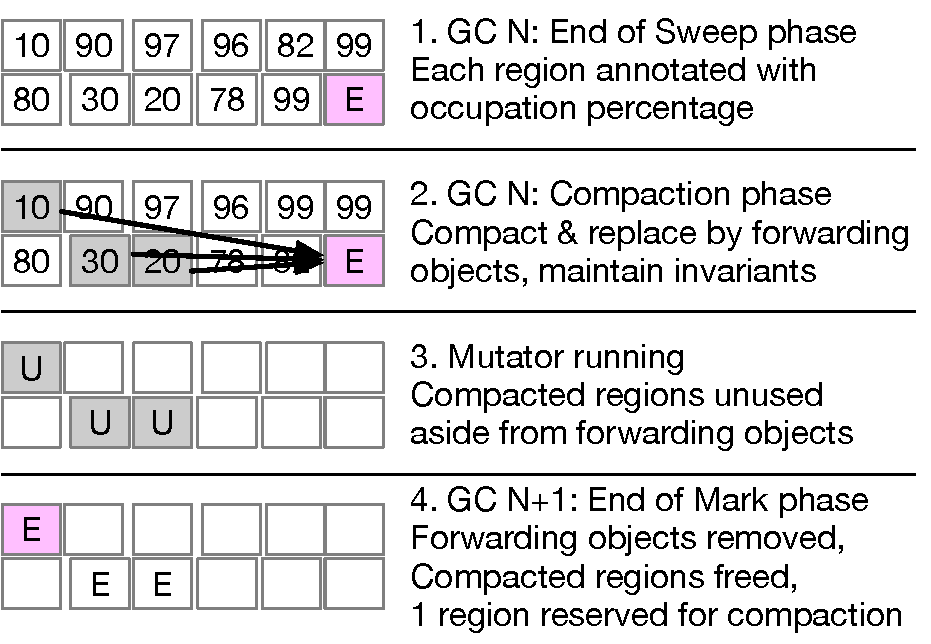
\includegraphics[width=.90\linewidth]{figures/SelectiveCompactFig} 
		\vspace{-0.3cm}
		\caption{Algorithm Summary\vspace{-0.3cm}}
		\label{fig:Algo}
 \end{figure}

\paragraph{Phase 1. End of Sweep Phase (Garbage Collection N).} We extended the existing sweep phase to compute the occupation of each memory region once scanned. 
Figure~\ref{fig:Algo} shows each region with its occupation as a percentage. 
In the common case, one region is empty and reserved from the previous garbage collection for the compaction phase, as detailed in the following paragraphs. 
This is depicted as a region E with a pink background.
%If no region is reserved, the VM allocates a new one, or throws an out of memory error during step 2.

%\egb{check whether you want VM or GC in this text. You used them both interchangeable. for example, I thought it is the algorithm which computes the regions to compact.}
\paragraph{Phase 2. Compaction Phase (Garbage Collection N).} The GC computes which memory regions to compact based on its occupancy. Regions are selected from the least occupied up until enough regions have been selected to fill up a reserved empty region to compact into. Regions which are more occupied than a threshold (70\% by default in our implementation) will not be compacted.
If all regions are almost full, the GC does not compact an almost full region into the region to compact into, but instead it skips entirely the compaction phase.
The GC ensures a memory region to compact into was reserved, otherwise it allocates a new one, or it aborts compaction if the allocation of a new memory region is impossible.

% if a segment is reserved to compact into, it removes its single large free chunk from the free chunk data structure. Alternatively, it allocates a new memory region (done at the first GC or after a non compacting GC) and and does the same thing.  
Once the regions to compact are selected, the VM iterates over all entities in all these regions. Found free chunks are removed from the free chunk structures so they cannot be allocated any more. Found objects are "moved" to the region to compact into; an object is moved by creating a copy of it in the region and mutating the original into a forwarding object pointing to the copy.
Last, the algorithm maintains the forwarding objects invariants.
%\egb{again, what the invariants entails is unclear here}

Figure~\ref{fig:Algo} shows that the algorithm selected the three least occupied regions (in gray) which are compacted into the reserved empty region (E with a pink background).

%\egb{unclear if this is the time between the end of compaction up to end of mark phase. Check first sentence of this paragraph for correctness}
\paragraph{Phase 3. Mutator Running.}  At the end of the compaction phase, all the compacted regions now contain only forwarding objects and the free chunks present inside them cannot be allocated. 
The mutator can run without using the compacted memory regions, aside from forwarding objects which are followed when met at runtime. In the figure, these regions are shown with the letter U (unoccupied, aside from forwarding objects).

\paragraph{Phase 4. End of Mark Phase (Garbage Collection N+1).} During the mark phase, the GC follows all forwarding objects. Memory regions marked as being compacted from the previous full GC can now be freed since they contained only forwarding objects, which are no longer referenced, and non allocatable free chunks. One of the unoccupied regions is reserved so that the next compaction phase can compact into it.

Figure~\ref{fig:Algo} shows that one of the F regions, now empty, is reserved (E with pink background) while the two others are also freed (E), but can be directly re-used by the VM. Once the sweep phase terminates, the algorithm goes back to phase 1.

\paragraph{Implementation Details.}
%In this paragraph we mention some details about our implementation. In 1., the sweep phase sets a 16 bits field in a small struct allocated for each region detailing its occupation (0 means unoccupied, 0xFFFF means fully occupied).  
In our implementation, the first (lowest) memory region is never selected for compaction since it contains kernel objects that the VM expects not to move. In addition, some memory regions may be marked as pinned, \ie they include objects which were requested by the program run not to move in memory. Pinned regions are also never compacted by our algorithm.%\footnote{This is by choice; of course we could compact the unpinned objects out of pinned regions to leave space for more pinned objects.  For now we are 0observing the KISS principle.}
%While compacting regions, the GC always iterates in ascending addresses order to ease free chunk management. Indeed, small free chunks are sorted to be removed efficiently since there is not enough room to implement a double linked lists within their fields. The GC sets up a free chunk from the remaining bytes left of the region to compact into, if any, at the end of this phase.

\subsection{Optimizing Forwarding Objects}

The original implementation of forwarding objects in~\cite{Forwarders} suffered from a significant overhead in
%in the interpreter and the template JIT, 
tight loops where each iteration of the loop requires to take a slow path to follow a forwarding object.
%which bodies are normally executed quickly, but require to follow a value at each iteration if a forwarding object is met. 
%Such loops induce significant overhead because the slow path to update the forwarding object is taken on each iteration. 

%The original 2015 design ~\cite{Forwarders} suffered from such cases.  

As a concrete example consider a method computing the sum of all the values present in an array passed as an argument. Figure \ref{fig:code} shows such an example. The code simply initializes the local variable \texttt{sum}, iterates over the array and add the value of the current item of the array to the sum. Lastly, the method answers the sum computed. 

\begin{figure}[bth]
		\vspace{-0.1cm}
\begin{verbatim}
sum: array
  | sum |
  sum := 0.
  1 to: array size do: 
    [:i | sum := sum + (array at: i)].
  ^ sum
\end{verbatim}
		\vspace{-0.3cm}
		\caption{Pathological Smalltalk Case\vspace{-0.3cm}}
		\label{fig:code}
 \end{figure}

The loop body is very simple and can be executed very quickly. The problem lies if the argument passed, \texttt{array}, is a forwarding object. Then, at each iteration of the loop, when performing the virtual call \texttt{at:} on the array\footnote{In Smalltalk, \texttt{+} and \texttt{at:} are normal virtual calls, which are resolved by the look-up logic to primitive methods.}, the partial read barrier of the cache logic fails and the VM executes code through a slow path to follow the forwarding object. Since the loop body is normally executed quickly, adding the overhead of a slow path drastically slow-down performance. 

When a virtual call to a forwarding object fails, the reference in the register to the forwarding object was always followed in the original implementation, so execution was always correct. But, if the register is loaded from memory at each iteration of the loop (which typically happens in the template JIT), the value in memory also needs to be followed. %We may think that a small loop like the one shown would keep the array in a register during the whole loop execution, and following the register would be enough. That is however not true in the interpreter and template JIT that we have in production since the loop body includes virtual calls. %A more aggressive optimizing JIT could partially solve that problem, but not entirely since loops require interrupt do better, but eventually the memory would need to be read again in other cases (recursions) or at least in 
% to avoid taking a slow path at each iteration of the loop. 
To solve this problem, existing heuristics would check, in addition to the register, if the local variables of the current stack frame and the literals of the current method executed were forwarding objects, and follow them too to avoid repeatedly following the same object and slowing down the loop.
 
In this work, we extended these heuristics to check for forwarding objects in the arguments of the current frame, the receiver's instance variables and specific instance variables of literals (to avoid getting a forwarding object when reading a global for example). The new heuristics successfully eliminated a source of slow down.

%Since all forwarding objects inducing overhead we found in the deployed applications we work on and the benchmarks discussed in the paper are covered by these new heuristics, we conclude that this optimization significantly reduced the overhead of forwarding objects. 
This optimization significantly reduced the overhead of forwarding objects since all forwarding objects inducing overhead we found in the deployed applications we work on and the benchmarks discussed in the paper are covered by the new heuristics.
Such an optimization is the key in achieving our second performance goal, which we will further discuss in the validation section.
 %We discuss further the execution time overhead of forwarding objects in the validation section.
 % the VM have  (typically, the VM patches a field in a heap object, in the arguments or temporary slots of the frame or in the literals of the method executed). Forwarding objects have been in production since 2015, such heuristics were tuned a lot during the past three years and we now believe that we cannot see the overhead of forwarding object in execution time on any deployed customer applications. 

\section{Validation}
\label{sec:validation}

%\egb{Rewrite glue text. "In this section we validate our work..." I want to read how you evaluate your work and not the meta. Give me the overview of experiments you conducted to validate your work}
In this section, we first give an overview of the validation and discuss the benchmarks we designed and built to evaluate our approach against our customer use-case. Then, we detail the methodology applied for the validation and our set-up. Next, we evaluate the distribution of compaction pauses on the benchmarks. We then show that forwarding objects do not impact execution time without GC. Lastly, we estimate the number of forwarding objects and references to them created during the GC compaction phase.

\subsection{Overview}
\label{sec:ow}

In this paper we claim that (1) not updating pointers during compaction pauses decreases significantly the pause times and (2) that the overhead introduced by the forwarding objects of our approach is very limited. To validate these claims, we need to compare our approach against another approach which updates pointers during the compaction pause and does not introduce forwarding objects similar to Garbage First \cite{G1}. 
%Such a competitive approach is very similar to Garbage First \cite{G1}. We however built our approach on top of existing work \cite{Forwarders}, re-using the same framework, \OpenSmalltalkVM. 
Since there is no such a thing as a Garbage First implementation in \OpenSmalltalkVM, we built a poor man's version of it. 
\footnote{One may wonder why the new algorithm was not implemented and evaluated in the JVM context, e.g. in Jikes RVM. We did not consider pursuing this evaluation strategy because (1) Jikes is currently 32 bits only, making it impossible to conduct experiments on the size of heaps we target (over 10 Gb), 
%forbidding the use of heaps over 10Gb for evaluation%and as such it is not possible to conduct experiments on the size of heaps we target in this paper
and (2) it does not feature the partial read barrier described in~\cite{Forwarders} we built upon, which would need to be re-implemented.}
In the next two paragraphs we briefly describe the two approaches compared, our approach, that we call lazy pointer update, and the competitive, Garbage First style approach, that we call eager pointer update.

\textbf{Lazy pointer update} is our approach where part of the heap is compacted during the compaction pause, but references to moved objects are updated lazily outside of the compaction pause. 

\textbf{Eager pointer update} emulates an implementation of the closest related work, i.e a Garbage First style approach where part of the heap is compacted but the references to moved objects are also updated during the compaction pause. Pointer update is performed using a per memory region remembered table. The table holds addresses of references from other memory regions to objects inside the region. Since this algorithm is used only as a reference, the remembered tables are computed during the compaction pause, and the time spent for their computation is then subtracted from the pause. In practice, they are implemented in Garbage First through fine-tuned write barriers that we could not easily emulate. We implemented eager pointer update in such a way because we believe it approximates a theoretical optimal pointer update phase in terms of execution time. %, \ie we believe the pointer update phase can hardly be quicker to execute that this implementation. 
Further details on the eager pointer update implementation are mentioned in Section \ref{sec:expPU}. 

%egb{following text cuts the flow and belongs to a discussion section if you want to keep it}
%One way to look at eager pointer update is that it first performs the lazy pointer update algorithm, then updates references to moved objects. Hence eager pointer update is necessarily worse in term of execution time than lazy pointer update.

\subsection{Benchmarks Built and Used}
%We worked on this GC algorithm in collaboration with a specific company using \OpenSmalltalkVM, \feenk\footnote{https://feenk.com/}, to decrease the GC pause time in their production application. Therefore, we designed and built benchmarks matching their exact use-case and evaluated the algorithm against it. As far as we know, they are the only user of \OpenSmalltalkVM 
The design of this GC algorithm is driven by the goal of decreasing garbage collection pauses in production applications using large heaps. One of this production application belongs to \feenk\footnote{https://feenk.com/}, a company building applications on \OpenSmalltalkVM using heaps up to 12Gb in production while needing a responsive environment. 

%\paragraph{Motivation.} We first look for benchmark suites dealing with heaps of similar size. 
To the best of our knowledge, existing VM benchmarks and even memory management intensive suites such as Dacapo \cite{DacapoBench} do not deal with the kind of targeted workloads (2 to 14Gb). Benchmark suites dealing with large workloads exist, such as Graph CHI \cite{GraphCHI}, but the workload is on disk, not in RAM. 

Within the Smalltalk community, the Squeak speed center\footnote{http://speed.squeak.org/} evaluates on a regular basis the performance of \OpenSmalltalkVM to track down performance regressions through 90 benchmarks. However, the benchmarks focus on the quality of the code generated by the just-in-time compiler and the scavenger (young space GC), none of the benchmark trigger multiple old space collections. Hence, these benchmarks were not appropriate to measure our algorithm, designed for the old space collector.

We therefore decided to build open-source benchmarks from the \feenk industrial use-case. The benchmarks built in such way are at least representative of one industrial use-case and target workloads of the sizes we are interested in.

%To validate our approach, we looked into other benchmark suites. In fact, other benchmarks are used to do performance analysis on the VM in the Squeak speed center\footnote{http://speed.squeak.org/}. However, the existing VM benchmarks and even memory management intensive suites such as Dacapo \cite{DacapoBench} do not deal with the kind of targeted workloads (2 to 14Gb). Benchmark suites dealing with large workloads exist, such as Graph CHI \cite{GraphCHI}, but the workload is on disk, not in RAM.

%SHORTER version

\paragraph{Benchmarks Built.} Part of the \feenk business includes the analysis of deployed industrial software to help solve specific problems in that software using the Moose software analysis framework~\cite{MooseBook1,MoosePaper1}. The analysed software is parsed into a graph of objects (up to 12Gb currently in production). Analysis can then be performed interactively on the graph of objects through small scripts (hence the need for responsiveness). The graph of objects is released once the analysis ends to free memory. 

We designed four main benchmarks, which can be used on different programs to analyse, \ie different workloads of different sizes. 
\begin{description}
	\item[Load:] The Load benchmark imports the software analysed into a graph of objects.
	\item[Exp:] The Exp benchmark expands properties, \ie it analyses the software with a frequently used set of analyses %, yields the analysis results 
	and caches some properties doing so.	
	\item[ExpCache:] The ExpCache benchmark is the same as Exp, but cached properties are already cached so they do not need to be recomputed and the heap is larger.
	\item[Release:] The Release benchmark releases the graph of objects and requests three garbage collections.
\end{description}

%In this section, we describe briefly the industrial use-case and how we designed and built the benchmarks from it. 
%Note that we did not use standard benchmark suites, not only because they do not match our customer use-case, but also because as far as we know they do not feature benchmarks with workload of a representative size for our use-case (\ie 2 to 14Gb). In Section \ref{sec:repBench}, we discuss further the representativity of the benchmark suite we built and compare it to other suites. 

%\paragraph{Industrial Use-case.} Part of the \feenk business includes analysing deployed industrial software to help solve specific problems in that software. Analyses are performed using the open-source Moose \cite{MooseBook1,MoosePaper1} framework, which supports analysing software written in different programming languages.
%To analyse software, the application in question is parsed into a graph of objects (up to 12Gb currently in production). Moose allows one to perform analysis on the model. Standard analyses are available and can be applied directly, but companies often request specific analyses matching their needs which have to be implemented in addition. During the analysis phase, some properties are computed repeatedly while other properties are computed once and then cached inside the model. Cached properties increase by up to a factor two the size of the model. Once the analyses are finished and the results produced, the model can be released, \ie all the components of the model are garbage collected.
%
%Software analysis is performed in an interactive framework, where one writes small scripts to analyse the model. One may wait for the result of the current script to perform the next one, or interrupt execution to see interim analysis results, or write the next script while the first one is running. Running the scripts and user interactions are currently performed in the same runtime, which is single-threaded, hence the need for responsiveness.
%
%\paragraph{Open-source Benchmarks.} The overall goal was to design open-source benchmarks from this industrial use-case. In particular, the benchmarks need to use workloads of similar size. 
%
%We faced three main issues while building the benchmarks. First, analysed softwares in the industrial use-case are closed-source. Second, analyses for customers are usually specific to their needs, and again closed-source. Third, Moose requires multiple parsers to analyse software written in multiple programming languages, and only a small subset of the parsers are open-source.
%We solve these problems by building benchmarks which, respectively, (1) analyse open-source programs of different sizes, (2) use a set of open-source analyses which is representative of frequently implemented analysis, and (3) use only the open-source version of one of the Java parsers.

%We also wanted to be able to show them publicly, \ie having them open-source. 

%COMPACTING TEXT
%The main issues we had were the following:
%\begin{enumerate}
%	\item Analysed softwares in the industrial use-case are closed-source (so far),
%	\item Analysis for customers are usually specific to their needs, different from standard analysis and closed-source, and
%	\item Moose requires multiple parsers to analyse a software written in multiple programming languages, and each parser has a different license (Some are open-source, some are closed-source).
%\end{enumerate}

%Each problem was solved respectively by building benchmarks which:
%\begin{enumerate}
%	\item Analyse open-source softwares of different sizes,
%	\item Use a set of open-source analysis which is representative to frequently implemented analysis, and
%	\item Use only the open-source version of one of the Java parser.
%\end{enumerate}
%\paragraph{Designed Benchmarks.} 

\paragraph{Workloads Used.} Since the benchmarks work with a program to analyse, the specific program analysed has an important impact on the benchmarks. Specifically, the size of the heap during the benchmarks is highly dependent on the size of the program analysed. In this paper, we ran the benchmarks with two Java projects, WildFly and NetBeans, which grow the heap from the base runtime of 300Mb to 3Gb and 14Gb respectively. Table \ref{tab:workloadSize} gives approximate workload sizes for the four benchmarks on the two projects. %SSIZE REDUCTION The Load benchmark grows the heap from 300Mb to respectively 2Gb and 8 Gb. The Exp benchmark grows the heap a bit more, to respectively 3Gb and 14Gb. The ExpCache benchmark does not change the size of the heap. The Release benchmark shrinks the heap back down to 300Mb.

\begin{table} [th]
\centering
\captionsetup{justification=centering}
\vspace{-0.2cm}
\caption{Approximate Workload sizes in Gb,\\
at the start and the end of each benchmark.\vspace{-0.2cm}}
\begin{tabular}{c|c|c|c|c}
   				& Load 			& Exp 		& \small{ExpCache}	& Release \\
	\hline
   	WildFly		& 0.3 $\rightarrow$ 2 	& 2 $\rightarrow$ 3	& 3 		& 3 $\rightarrow$ 0.3 \\
   	NetBeans		& 0.3 $\rightarrow$ 8 	& 8 $\rightarrow$ 14 	& 14 		& 14 $\rightarrow$ 0.3 \\
%Actual data: workload an Array(302653440 a GCMooseBench 8 355 717 120 a GCMooseBench 14 261 297 152)
\end{tabular} 
\vspace{-0.4cm}
\label{tab:workloadSize}
\end{table}

\subsection{Methodology and Set-up}

\def\numRuns{30\xspace}

%\paragraph{Hardware and OS.}
The benchmarks were run in parallel on 10 nodes of the same cluster, each node having the exact same specifications. Each node is a HP ProLiant DL20 Gen9, with a Intel Xeon CPU E3-1240 v5 (3.5 GHz) and has 32 Gb of RAM. The OS installed on each node is Ubuntu 16.04.5 LTS (GNU/Linux 4.4.0-133-generic x86\_64). Although each node has four cores, we ran only one benchmark at a time on each node, to avoid exhausting available RAM and suffering paging side-effects.

%\paragraph{\OpenSmalltalkVM.}
The benchmarks were run on a custom compiled version of the \OpenSmalltalkVM, derived from version 2419 of VMMaker. The two differences compared to the open-source production VM is that we added (1) performance analysis features to compute exact pause times and (2) the eager pointer update algorithm. 
%Both features did not make it to production and are not on the repository. %\eem{Why not?  It would be good to have this available somewhere :-)} 
%\egb{you lost me: is it in production or not, why you just put a url to the repo and that's all}
The lazy pointer update algorithm is in the production VM under the name "SpurSelectiveCompactor". 
Note that the \OpenSmalltalkVM features an interpreter and a template JIT, which provides strong baseline performance, but does not feature a JIT performing speculative optimizations. We discuss the side-effects of the lack of a speculative optimizer later in Section \ref{sec:optJITDisc}.

%\paragraph{Runs.}
To obtain results, we ran each benchmarks for each configuration \numRuns times, 3 times on each node. Benchmarking with the NetBeans workload takes a significant amount of time (around 4 hours per benchmark, on an evaluation with 2 configurations that gives us a total of 240 hours total cpu time, 24h on each node).
%, we did not run the benchmarks more times to avoid wasting resources. 

\subsection{Compaction Pause Time Experiments}

%\paragraph{Experiments.}
In this experiment, for each benchmark we measured the compaction pause of each full garbage collection pause. In the context of lazy pointer update, the pause is composed mainly of the time spent compacting the selected memory regions, the rest (maintaining the invariants, etc.) represents a very small fraction of the pause. In eager pointer update, the pause includes in addition the time updating the pointers in the heap.

\paragraph{Measurements.}
We extended the GC for this experiment to store in a buffer the UTC\footnote{Coordinated Universal Time} time in micro seconds at the start and the end of the compaction phase. In lazy pointer update, these two time stamps are the only values recorded. In eager pointer, the implementation used is required to compute a remembered table in between the phase where objects are moved and the phase where pointer are updated, as discussed further in Section \ref{sec:expPU}. The time computing the remembered tables is irrelevant in the context of fine-tuned high performance write barriers which maintain such remembered tables. Hence, we compute four time stamps in this case to compute the compaction pause and subtract the time spent computing the remembered table from it.

\newcommand{\rulesep}{\unskip\ \vrule\ }

\begin{figure*}[bth]
	\centering
	\rotatebox{90}{\hspace{2.2cm}\footnotesize{Compaction pauses in ms}}
	\begin{subfigure}[b]{.48\textwidth}
    	\begin{subfigure}[b]{.24\textwidth}
		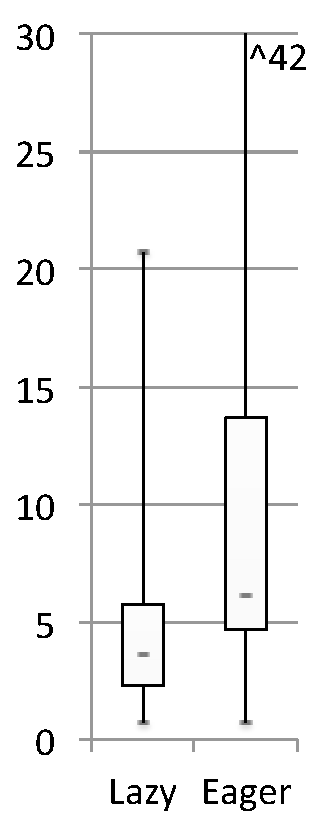
\includegraphics[width=\linewidth]{figures/netBeansLoad} 
		\caption{Load}
   	\end{subfigure}% 
   	\begin{subfigure}[b]{.24\textwidth}
		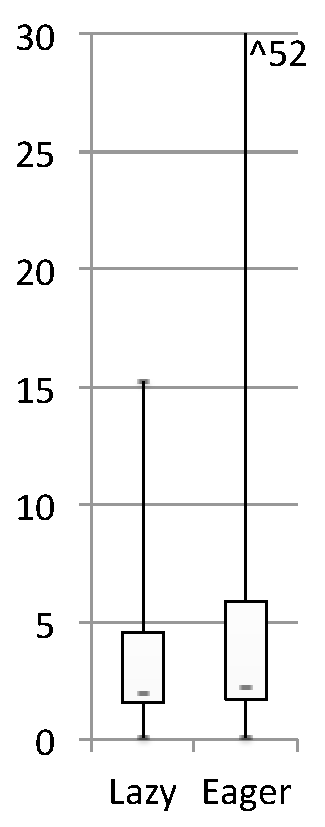
\includegraphics[width=\linewidth]{figures/netBeansExp} 
		\caption{Exp}
   	\end{subfigure}	
	\begin{subfigure}[b]{.24\textwidth}
		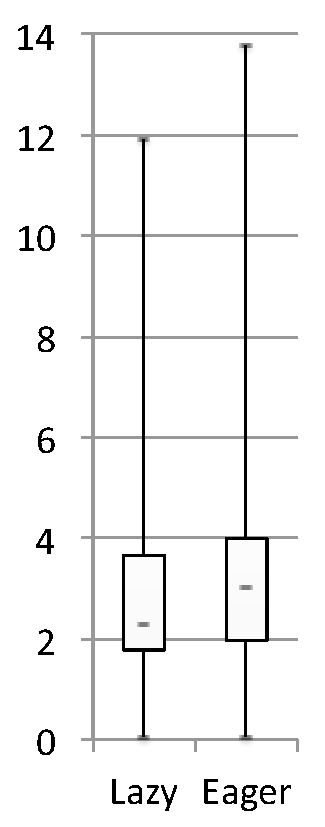
\includegraphics[width=\linewidth]{figures/netBeansExpCache} 
		\caption{ExpCache}
	\end{subfigure}%
	\begin{subfigure}[b]{.24\textwidth}
		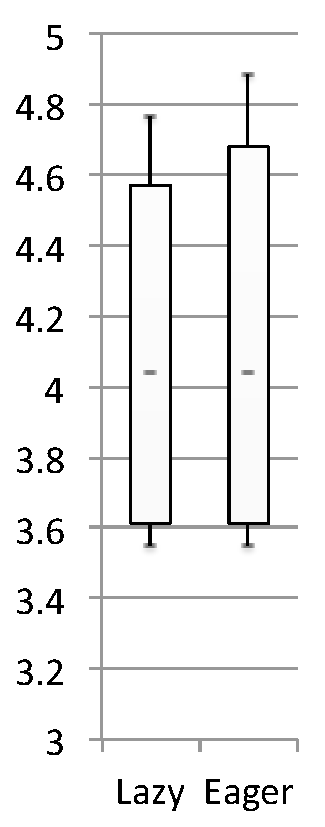
\includegraphics[width=\linewidth]{figures/netBeansRelease} 
		\caption{Release}
   	\end{subfigure}%
	\caption*{NetBeans 14 Gb Workload}
	\end{subfigure}%
	\rotatebox{90}{\hspace{2.2cm}\footnotesize{Compaction pauses in ms}}
	\begin{subfigure}[b]{.48\textwidth}
    	\begin{subfigure}[b]{.24\textwidth}
    		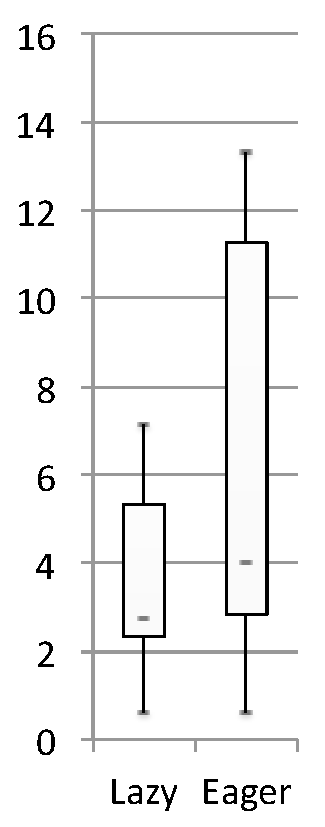
\includegraphics[width=\linewidth]{figures/wildflyLoad} 
    		\caption{Load}
       	\end{subfigure}% 
       	\begin{subfigure}[b]{.24\textwidth}
    		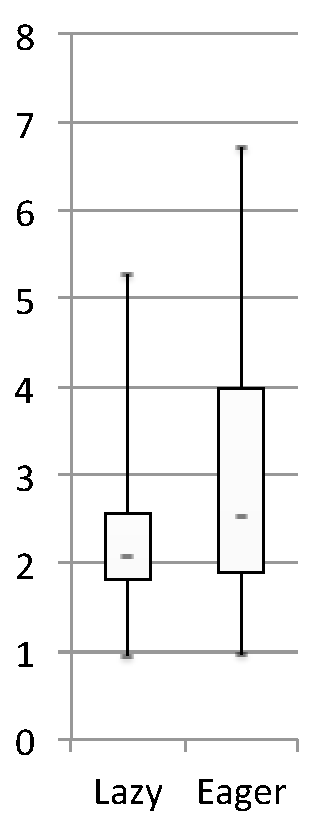
\includegraphics[width=\linewidth]{figures/wildflyExp} 
    		\caption{Exp}
       	\end{subfigure}	
    	\begin{subfigure}[b]{.24\textwidth}
    		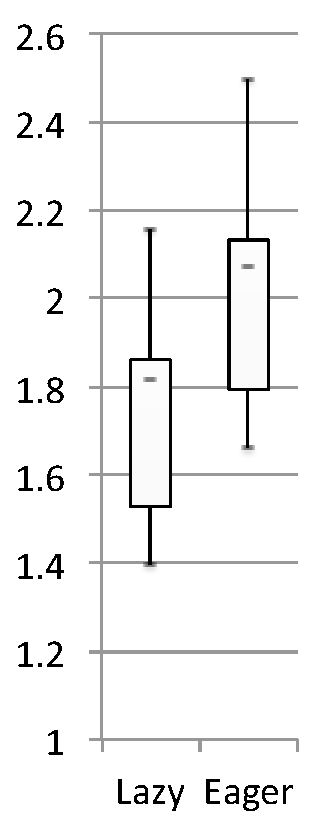
\includegraphics[width=\linewidth]{figures/wildflyExpCache} 
    		\caption{ExpCache}
    	\end{subfigure}%
    	\begin{subfigure}[b]{.24\textwidth}
    		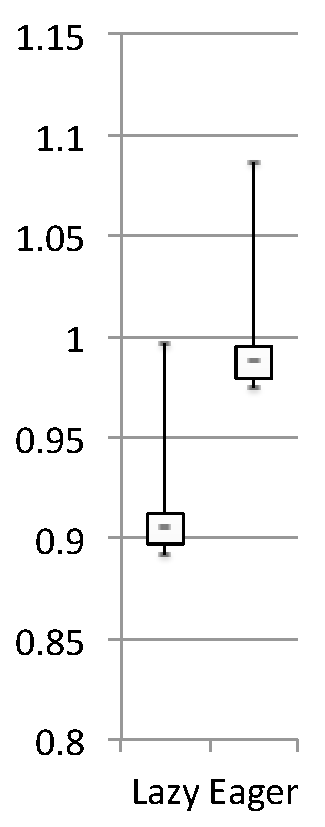
\includegraphics[width=\linewidth]{figures/wildflyRelease} 
    		\caption{Release}
   	\end{subfigure}   
	\caption*{WildFly 3 Gb Workload}
	\end{subfigure}	   
	\vspace{-0.8cm}
	\caption{Compaction pauses\vspace{-0.2cm}}
	\label{fig:compactPause}
\end{figure*}

\begin{table*} [ht]
\centering
\caption{Compaction pauses (All values in $\mu$s)\vspace{-0.2cm}}
\resizebox{\textwidth}{!}{%
\begin{tabular}{c|c|r|r|c|r|r|r|r|r|r}
	 \multirow{2}{*}{\small{Workload}} 	& \multirow{2}{*}{\small{Benchmark}} & \small{GC}		& \small{Comp.	} 	& \small{Pointer} 	& \small{First}		& \multirow{2}{*}{\small{Min}} 	&  \multirow{2}{*}{\small{Median}} 	& \multirow{2}{*}{\small{Max}} 	& \small{Third} 		& \small{Average $\pm$}	 \\
								&					      		&  \small{per run}	& \small{per run} 	& \small{Update}	& \small{Quartile}	& 				  		& 					 		& 				    		& \small{Quartile} 	& \small{Std Deviation} 	\\
	\hline
	\multirow{8}{*}{\small{NetBeans}}	& \multirow{2}{*}{\small{Load}} 		& \multirow{2}{*}{23} 		& \multirow{2}{*}{19}  	& \small{Lazy}	& 2292	& 679			& 3673	& 20697	& 5747		& 4779 $\pm$ 4163	 \\
								&							& 					&				  	& \small{Eager}	& 4691	& 679			& 6128	& 42318	& 13677		& 9418 $\pm$ 8761	 \\
								& \multirow{2}{*}{\small{Exp}} 		& \multirow{2}{*}{81} 		& \multirow{2}{*}{67}  	& \small{Lazy}	& 1588	& 84				& 1929	& 15245	& 4563		& 3288 $\pm$ 2708	 \\
								&							& 					&				  	& \small{Eager}	& 1720	& 84				& 2194	& 52213	& 5886		& 4296 $\pm$ 4942	 \\
								& \multirow{2}{*}{\small{ExpCache}} 	& \multirow{2}{*}{96} 		& \multirow{2}{*}{88}  	& \small{Lazy}	& 1776	& 51				& 2287	& 11894	& 3651		& 2872 $\pm$ 1873	 \\
								&							& 					&				  	& \small{Eager}	& 1973	& 51				& 3002	& 13751	& 3991		& 3491 $\pm$ 2330	 \\
								& \multirow{2}{*}{\small{Release}} 	& \multirow{2}{*}{3} 		& \multirow{2}{*}{3}  		& \small{Lazy}	& 3613	& 3551			& 4040	& 4765	& 4572		& 4140 $\pm$ 471	\\
								&							& 					&				  	& \small{Eager}	& 3613	& 3551			& 4040	& 4886	& 4680		& 4195 $\pm$ 524	 \\
	\hline
	\multirow{8}{*}{\small{WildFly}}	& \multirow{2}{*}{\small{Load}} 		& \multirow{2}{*}{12} 		& \multirow{2}{*}{12}  	& \small{Lazy}	& 2326	& 603			& 2746	& 7133	& 5338		& 3530 $\pm$ 1838 	 \\
							&							& 					&				  	& \small{Eager}	& 2832	& 610			& 3993	& 13347	& 11275		& 6315 $\pm$ 4336 	 \\
							& \multirow{2}{*}{\small{Exp}} 		& \multirow{2}{*}{9} 		& \multirow{2}{*}{8}  		& \small{Lazy}	& 1811	& 954			& 2082	& 5269	& 2566		& 2308 $\pm$ 1191 	 \\
							&							& 					&				  	& \small{Eager}	& 1895	& 970			& 2536	& 6714	& 3981		& 3059 $\pm$ 1714 	 \\
							& \multirow{2}{*}{\small{ExpCache}} 	& \multirow{2}{*}{5} 		& \multirow{2}{*}{5}  		& \small{Lazy}	& 1528	& 1396			& 1816	& 2158	& 1861		& 1726 $\pm$ 192	 \\
							&							& 					&				  	& \small{Eager}	& 1794	& 1662			& 2071	& 2497	& 2133		& 1999 $\pm$ 203	 \\
							& \multirow{2}{*}{\small{Release}} 	& \multirow{2}{*}{3} 		& \multirow{2}{*}{2}  		& \small{Lazy}	& 897	& 892			& 905	& 996	& 912		& 912 $\pm$ 24	 \\
							&							& 					&				  	& \small{Eager}	& 979	& 975			& 988	& 1086	& 995		& 998 $\pm$ 28 	 \\

	\end{tabular} }
\label{tab:compactPause}
\vspace{-0.3cm}
\end{table*}


%\begin{table*} [ht]
%\centering
%\caption{Compaction pauses (All values in $\mu$s)\vspace{-0.2cm}}
%\resizebox{\textwidth}{!}{%
%\begin{tabular}{c|c|r|r|c|r|r|r|r|r|r|r}
%	 \multirow{2}{*}{\small{Workload}} 	& \multirow{2}{*}{\small{Benchmark}} & \small{GC}		& \small{Comp.	} 	& \small{Pointer} 	& \small{First}		& \multirow{2}{*}{\small{Min}} 	&  \multirow{2}{*}{\small{Median}} 	& \multirow{2}{*}{\small{Max}} 	& \small{Third} 		& \small{Average $\pm$}	& \small{Outliers} \\
%								&					      		&  \small{per run}	& \small{per run} 	& \small{Update}	& \small{Quartile}	& 				  		& 					 		& 				    		& \small{Quartile} 	& \small{Std Deviation} 	& \small{\textgreater16.6ms}\\
%	\hline
%	\multirow{8}{*}{\small{WildFly}}	& \multirow{2}{*}{\small{Load}} 		& \multirow{2}{*}{12} 		& \multirow{2}{*}{12}  	& \small{Lazy}	& 2326	& 603			& 2746	& 7133	& 5338		& 3530 $\pm$ 1838 	& 0 \\
%							&							& 					&				  	& \small{Eager}	& 2832	& 610			& 3993	& 13347	& 11275		& 6315 $\pm$ 4336 	& 0 \\
%							& \multirow{2}{*}{\small{Exp}} 		& \multirow{2}{*}{9} 		& \multirow{2}{*}{8}  		& \small{Lazy}	& 1811	& 954			& 2082	& 5269	& 2566		& 2308 $\pm$ 1191 	& 0 \\
%							&							& 					&				  	& \small{Eager}	& 1895	& 970			& 2536	& 6714	& 3981		& 3059 $\pm$ 1714 	& 0 \\
%							& \multirow{2}{*}{\small{ExpCache}} 	& \multirow{2}{*}{5} 		& \multirow{2}{*}{5}  		& \small{Lazy}	& 1528	& 1396			& 1816	& 2158	& 1861		& 1726 $\pm$ 192	& 0 \\
%							&							& 					&				  	& \small{Eager}	& 1794	& 1662			& 2071	& 2497	& 2133		& 1999 $\pm$ 203	& 0 \\
%							& \multirow{2}{*}{\small{Release}} 	& \multirow{2}{*}{3} 		& \multirow{2}{*}{2}  		& \small{Lazy}	& 897	& 892			& 905	& 996	& 912		& 912 $\pm$ 24	& 0 \\
%							&							& 					&				  	& \small{Eager}	& 979	& 975			& 988	& 1086	& 995		& 998 $\pm$ 28 	& 0 \\
%	\hline
%	\multirow{8}{*}{\small{NetBeans}}	& \multirow{2}{*}{\small{Load}} 		& \multirow{2}{*}{23} 		& \multirow{2}{*}{19}  	& \small{Lazy}	& 2292	& 679			& 3673	& 20697	& 5747		& 4779 $\pm$ 4163	& 6 \\
%								&							& 					&				  	& \small{Eager}	& 4691	& 679			& 6128	& 42318	& 13677		& 9418 $\pm$ 8761	& 6 \\
%								& \multirow{2}{*}{\small{Exp}} 		& \multirow{2}{*}{81} 		& \multirow{2}{*}{67}  	& \small{Lazy}	& 1588	& 84				& 1929	& 15245	& 4563		& 3288 $\pm$ 2708	& 0 \\
%								&							& 					&				  	& \small{Eager}	& 1720	& 84				& 2194	& 52213	& 5886		& 4296 $\pm$ 4942	& 9 \\
%								& \multirow{2}{*}{\small{ExpCache}} 	& \multirow{2}{*}{96} 		& \multirow{2}{*}{88}  	& \small{Lazy}	& 1776	& 51				& 2287	& 11894	& 3651		& 2872 $\pm$ 1873	& 0 \\
%								&							& 					&				  	& \small{Eager}	& 1973	& 51				& 3002	& 13751	& 3991		& 3491 $\pm$ 2330	& 0 \\
%								& \multirow{2}{*}{\small{Release}} 	& \multirow{2}{*}{3} 		& \multirow{2}{*}{3}  		& \small{Lazy}	& 3613	& 3551			& 4040	& 4765	& 4572		& 4140 $\pm$ 471	& 0 \\
%								&							& 					&				  	& \small{Eager}	& 3613	& 3551			& 4040	& 4886	& 4680		& 4195 $\pm$ 524	& 0 \\
%	\end{tabular} }
%\label{tab:compactPause}
%\vspace{-0.3cm}
%\end{table*}

\paragraph{Results.} 
The compaction pauses measured on the two workloads and the four benchmarks, for lazy and eager pointer update, are displayed in Table \ref{tab:compactPause} and Figure \ref{fig:compactPause}. 
Table  \ref{tab:compactPause} shows for each benchmark the average number of full garbage collection per run. Since there were \numRuns runs, one needs to multiply that number by \numRuns to get the total number of pauses considered in the evaluation. A compaction phase starts during a full garbage collection only if at least one memory segment is less than 70\% occupied. The next column in the table indicates the average number of compactions performed per run, which can be lower than the total number of full garbage collections. The following columns indicate the first quartile, min, median, max and third quartile of the compaction pauses measured.  Figure \ref{fig:compactPause} includes whisker charts drawn using these five values. Table \ref{tab:compactPause} also includes the computed average pause and the standard deviation.%, though in the context of pauses we are mainly interested in the median, third quartile and max pause. %The last columns details the number of compaction pauses above our performance goal, 16.6ms.

%\paragraph{Analysis.} 
In the Load and Exp benchmarks, the heap grows considerably. In this context it seems the number of inter-region references is higher and the difference between lazy and eager pointer update is large, especially in the context of the maximum pause and the third quartile. Growing to 8Gb and then to 14Gb in NetBeans shows maximum compaction pauses up to three times longer with eager pointer update. In the ExpCache benchmark, when the heap size remains stable, the number of inter-region references look lower and the difference between lazy and eager pointer update is minimal (up to 2ms difference in the worst case, median is up to 0.7ms worse). In the Release benchmark, inter-region references are rare since the heap is shrinking from either 14Gb or 3Gb down to 300Mb. A few full garbage collections are enough to shrink the heap in these cases. Most segments are entirely empty, leading the first garbage collection to shrink the heap by freeing over a hundred segments, but some objects, including for example objects related to process scheduling remain. It takes therefore two full garbage collections to free these segments (they are freed at the end of the marking phase of the next garbage collection).

%\egb{this makes it sound bad, as if you built the benchmark only for the algo}
%\paragraph{Discussion.} 
In our context, we tried to find compaction pauses where the pointer update phase represents more than 20\% of the compaction pause time, making it relevant to move that phase away from the compaction pause. In these benchmarks, with these workloads, not updating the pointers reduces the median pause up to \bestMedian and the longest pause up to \bestWorst. 

In the WildFly workload, the Load and Exp benchmarks have worst pauses that are 47\% and 22\% smaller with lazy pointer update. In the Load benchmark, the median pause is even 32\% smaller without updating the pointers. In the NetBeans workload, the Load and Exp benchmarks have worst pauses 51\% and 71\% smaller with lazy pointer update. The Load and ExpCache benchmark even have median pause 41\% and 24\% smaller without updating the pointers. A considerable amount of compaction pauses therefore benefit from lazy pointer update in these benchmarks, and we conclude that our first performance goal is met.

%the performance goal is met by the two algorithms. However, in the Load benchmark the eager pointer update worst pause is 13.3ms and the third quartile is at 11.3ms. Such pauses are quite close to the limit, which means that on a less powerful machine (the benchmarking machine has 3.5GHz), the 16.6ms threshold is likely to be reached. Lazy pointer update caps however at 7.1ms pause for the same benchmark.

%the performance goal is met by both algorithms for the ExpCache and Release benchmark. Only lazy pointer update meets the goal for the Exp benchmark, while eager pointer update has 9 outlying values up to 52.2ms. In the case of the Load benchmark, none of the benchmarks meet the performance goal with 6 outlying values each. However, with lazy pointer update, the worst pause is significantly better with 20.7ms instead of 42.3ms. In addition, lazy pointer update has a third quartile at 5.7ms instead of 13.6ms. This likely means that on slower machines still a small number of pauses would exceed the threshold with lazy pointer update, while with eager pointer update one quarter of the pauses can potentially exceed the performance goal.

\subsection{Execution Time Experiments}

\begin{figure*}[bth]
	\centering
	\begin{subfigure}[b]{.48\textwidth}
	\rotatebox{90}{\hspace{1.2cm}\footnotesize{Execution time in seconds}}
    	\hspace{.03\textwidth}\begin{subfigure}[b]{.28\textwidth}
		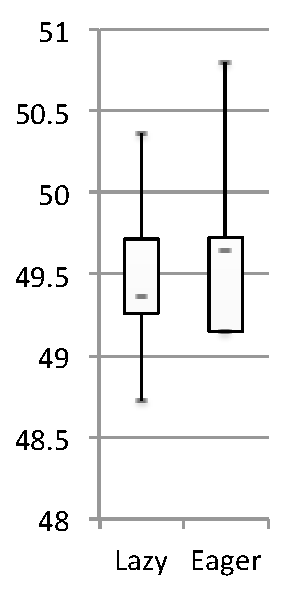
\includegraphics[width=\linewidth]{figures/netBeansLoadExecTime} 
		\caption{Load}
   	\end{subfigure}\hspace{.03\textwidth}% 
   	\begin{subfigure}[b]{.28\textwidth}
		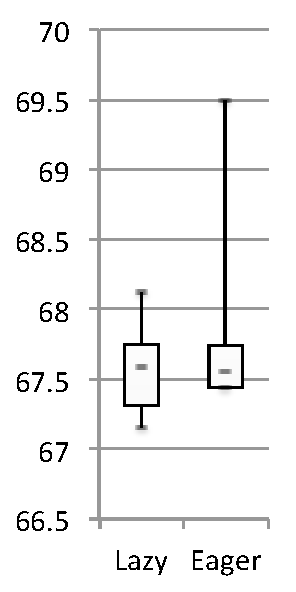
\includegraphics[width=\linewidth]{figures/netBeansExpExecTime} 
		\caption{Exp}
   	\end{subfigure}\hspace{.03\textwidth}% 
	\begin{subfigure}[b]{.28\textwidth}
		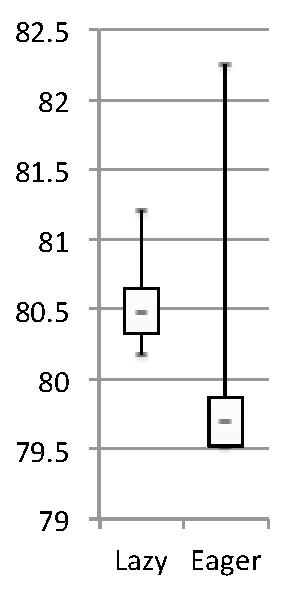
\includegraphics[width=\linewidth]{figures/netBeansExpCacheExecTime} 
		\caption{ExpCache}
	\end{subfigure}%
	\caption*{WildFly 3 Gb Workload\vspace{-0cm}}
	\end{subfigure}%
	\begin{subfigure}[b]{.48\textwidth}
	\rotatebox{90}{\hspace{1.2cm}\footnotesize{Execution time in seconds}}
    	\hspace{.03\textwidth}\begin{subfigure}[b]{.28\textwidth}
    		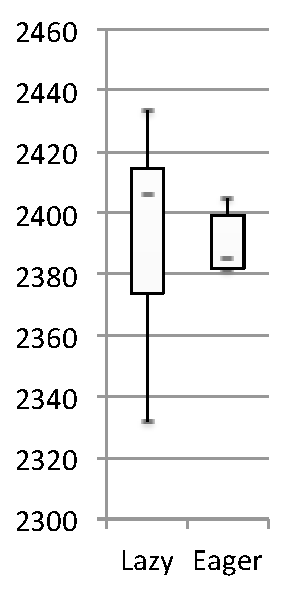
\includegraphics[width=\linewidth]{figures/wildflyLoadExecTime} 
    		\caption{Load}
       	\end{subfigure}\hspace{.03\textwidth}% 
       	\begin{subfigure}[b]{.28\textwidth}
    		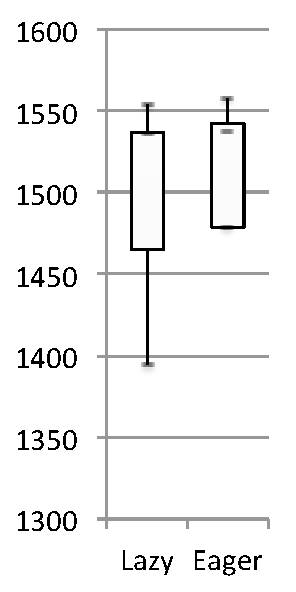
\includegraphics[width=\linewidth]{figures/wildflyExpExecTime} 
    		\caption{Exp}
       	\end{subfigure}\hspace{.03\textwidth}% 
    	\begin{subfigure}[b]{.28\textwidth}
    		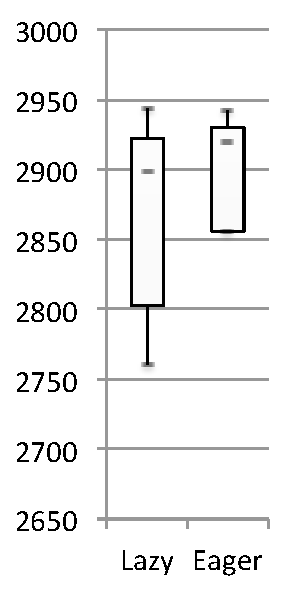
\includegraphics[width=\linewidth]{figures/wildflyExpCacheExecTime} 
    		\caption{ExpCache}
    	\end{subfigure}%  
	\caption*{NetBeans 14 Gb Workload\vspace{-0cm}}
	\end{subfigure}	   
	\vspace{-0.3cm}
	\caption{Execution time without GC\vspace{-0.2cm}}
	\label{fig:execTime}
\end{figure*}

\begin{table*} [bht]
\centering
\caption{Execution time\vspace{-0.2cm}}
\begin{tabular}{c|c|c|r|r|r|r|r|r}
	 \multirow{2}{*}{Workload} & \multirow{2}{*}{Benchmark} 	& Pointer  		& First			& \multirow{2}{*}{Min} &  \multirow{2}{*}{Median} & \multirow{2}{*}{Max} & Third 		& Average $\pm$ \\
						&					      	& Update 		& \small{Quartile}	& 				  & 					  & 				    & \small{Quartile} 	& \small{Std Deviation} \\
	\hline
						& \multirow{2}{*}{Load} 	 	& Lazy		& 2373	& 2331	& 2406	& 2433 & 2414	& 2398 $\pm$ 29.6 \\
						&						& Eager		& 2381	& 2381	& 2384	& 2404 & 2399	& 2394 $\pm$ 9.40 \\
	NetBeans				& \multirow{2}{*}{Exp} 		& Lazy		& 1464	& 1394	& 1536	&1554  & 1537	& 1509 $\pm$ 51.7 \\
	\small{Values in s}		&					  	& Eager		& 1478	& 1478	& 1536	& 1557 & 1542	& 1532 $\pm$ 27.6 \\
						& \multirow{2}{*}{ExpCache}	& Lazy		& 2802	& 2759	& 2898	& 2943 & 2922	& 2876 $\pm$ 63.4 \\
						&					  	& Eager		& 2855	& 2855	& 2919	& 2942 & 2929	& 2916 $\pm$ 31.4 \\
	\hline
						& \multirow{2}{*}{Load} 	 	& Lazy		& 49262	& 48723			& 49363	& 50361	& 49716		& 49560 $\pm$ 450 \\
						&						& Eager		& 49149	& 49149			& 49649	& 50796	& 49723		& 49560 $\pm$ 507 \\
	WildFly				& \multirow{2}{*}{Exp} 		& Lazy		& 67309	& 67150			& 67592	& 68128	& 67747		& 67637 $\pm$ 294 \\
	\small{Values in ms}	&					  		& Eager		& 67438	& 67438			& 67550	& 69495	& 67743		& 67979 $\pm$ 700\\
						& \multirow{2}{*}{ExpCache} 	& Lazy		& 80324	& 80169			& 80476	& 81197	& 80648		& 80617 $\pm$ 314 \\
						&					  	& Eager		& 79522	& 79522			& 79704	& 82254	& 79871		& 80418 $\pm$ 1130 \\
	\end{tabular} 
\label{tab:execTimeTable}
\vspace{-0.1cm}
\end{table*}

%\paragraph{Context.}
The original implementation of forwarding objects in \cite{Forwarders} relied on forwarding objects to be uncommon to avoid overhead on execution time. In that work, forwarding objects were met at runtime exclusively when created from the Smalltalk \emph{become} primitive. 
%\egb{the following sentence says the same as the following one. So I removed it.}
%If forwarding objects become common as it is the case in this work, the runtime may be slowed down since common operations are more likely to fail because a forwarding object has to be followed. 
Since our algorithm creates a higher number of forwarding objects that we had ever seen before in production applications,
%\footnote{Forwarding objects were met at runtime exclusively when created from the Smalltalk \emph{become} primitive before this GC implementation.}
we re-evaluated the forwarding object overhead. 
As explained in the previous section, we extended the VM so that when a forwarding object is followed, the memory location where the forwarding object came from (receiver instance variables, literals, arguments or temporary variables) is immediately followed. 
%\egb{very careful here. you have not evaluated the optimization separately, so I removed the details.}
%to avoid the pathological case of a tight loop getting very slow at each iteration. These optimizations also needed to be evaluated.%\eem{But I still don't see this not happening in default Spur :-(; we need to look carefully and you can show me what to look for}

\paragraph{Measurements.}
In this experiment, we ran our benchmarks with lazy and eager pointer update, but we compare execution time without GC instead of compaction pauses. We did not calculate the execution time of the Release benchmark since the benchmark only sets a variable to nil before running the garbage collector three times (execution time without garbage collection is always below 10$\mu$s and irrelevant). The production \OpenSmalltalkVM records by default the time spent in scavenges and full garbage collections. The results shown are computed from the total execution time, to which the total time spent in scavenges and full garbage collections have been subtracted.

\paragraph{Results.}
Table \ref{tab:execTimeTable} and Figure \ref{fig:execTime} show the results. Median, worst and average execution time between eager and lazy pointer update are within 1\% performance difference from each other. We therefore conclude based on these results that the higher number of forwarding objects has no significant impact on execution time of the application, excluding garbage collection time. As such, we also met the second performance goal.

\subsection{Approximate Number of Forwarding Objects}

In this experiment, we ran the same benchmarks as the previous subsection with the WildFly workload. We counted the number of forwarding objects created by the compaction algorithm (sum of the number of forwarding objects present at the end of each GC). We counted the number of old space collection including a compaction phase. We estimated the number of forwarding objects created by each compaction pause (Total number of forwarding objects created in the benchmark divided by number of old space collection with a compaction phase). We evaluated the number of objects on heap at the beginning and end of each benchmark. We counted the number of references updated at runtime through partial read barrier failures during the benchmark and counted the total number of references to update because they refer to forwarding objects created by the compaction algorithm (sum of the number of references to forwarding objects present at the end of each GC). Table \ref{tab:numFwd} summarizes the results found. 

\begin{table*} [bht]
\centering
\caption{Number of Forwarding Objects Created and References Updated in the WildFly Workload (\small{Average $\pm$ Std Deviation})\vspace{-0.2cm}}
\begin{tabular}{c|c|r|r|r|r|r|r}
	 \multirow{4}{*}{\small{Benchmark}} 	  		& \small{Number of} 			& \small{Number} 			& \small{Approx. Number} 	& \small{Number of}			& \small{Number of}			& \small{Refs }				&  \small{Total } \\
						      	 			& \small{Forwarding}			& \small{of}				& \small{of Forwarding} 		& \small{Objects at}			& \small{Objects at}			& \small{Updated}			& \small{Refs} \\
						      	 			& \small{Objects}			& \small{Compacting}		& \small{Objects Created} 	& \small{Start-up}		& \small{Shut-down}			& \small{at}				& \small{to} \\
						      	 			& \small{Created}			& \small{GCs}				& \small{per Compacting GC} 	& \small{(millions)}			& \small{(millions)}				& \small{Runtime}			& \small{Update} \\
	\hline
	 \small{Load}	 						& \small{1777670 $\pm$ 19768	}	& 12 					& ~148139				& 3 		& 16				& \small{627909 $\pm$ 9706}		& \small{2548602 $\pm$ 29793} \\			
	 \small{Exp} 					 		& \small{119443 $\pm$ 21809}		& 8 					& ~14930					& 16 		& 21				& \small{2394 $\pm$ 951}			& \small{120278	$\pm$ 22015} \\
	 \small{ExpCache}						& \small{39027 $\pm$ 24256} 		& 5 					& ~7805					& 21 		& 21				& \small{563 $\pm$ 1112}			& \small{39027 $\pm$ 24256} \\
\end{tabular} 
\label{tab:numFwd}
\vspace{-0.3cm}
\end{table*}

\paragraph{Results.} In the Load benchmark, 1.78 millions of forwarding objects are created across 12 GCs. 2.55 millions of references needs to be updated across the benchmark to avoid referencing forwarding objects. In the case of eager pointer update, the time spent updating these references is spread across the twelve compaction pauses. In the case of lazy pointer update, 628 thousands of references are updated lazily when met at runtime, while the rest of the references are updated through the next GC marking phase. The Load benchmark is specific because almost one quarter of the references are updated at runtime with our algorithm, lazy pointer update. In the two other benchmarks, most references to forwarding objects are unused at runtime: they are updated by the following GC marking phase before being accessed. This makes sense since for example in the ExpCache benchmark the heap contains around 21 millions objects and only approximately 8 thousands of them (0.038\%) are converted to forwarding object on compaction pauses.

\paragraph{Execution Time Overhead.} We estimated with a micro-benchmark that the time spent updating a forwarding object met at runtime to an order of magnitude of ten nanoseconds. More concretely, it  accounts the time spent exiting the code generated by the JIT to go to C code due to the forwarding object met, executing the C code to follow with heuristics fields of different objects to avoid looping repeatedly on the same forwarding object and lastly resuming execution of the code generated by the JIT. Even in the Load benchmark, where 628 thousands of references are updated lazily when met at runtime, the total execution time overhead of such updates is estimated to 6 milliseconds in a benchmark taking approximately 49.5 seconds and a standard deviation of 500 milliseconds. The overhead of lazy update is therefore negligible and hard to see in the total execution time without GC of the benchmark.


\section{Threats to Validity and Discussion}
\label{sec:threats}

We believe the validation is very strong, but specific concerns may threaten its validity: the representativity of our benchmarks, the experimental eager pointer update implementation and the compaction heuristics. These aspects are detailed in this section. Then, we discuss the memory pressure of the compacting algorithm and the applicability of our approach to other VMs.

\subsection{Threats to Validity}

\paragraph{Benchmarks Representativity.} 
\label{sec:repBench}
The first threat to validity is how representative our benchmarks are to production applications. Given how we designed and build our benchmarks, they are representative of at least one industrial deployed application. 
%However, few industrial users need both a responsive runtime and a large heap. 
%Most of our them deploy web services with runtimes less than 300 Mb. 
%Among large heaps users, some of them perform long running analysis which do not require the runtime to be responsive. 
%REDUC DLS
%However, the benchmarks built may not cover all the possible large production workloads. For example, another \OpenSmalltalkVM company is doing proofs on state machines, having multi Gb heaps holding mainly machine states in huge byte arrays. However, huge objects are not moved by our GC (because they are typically the only object in their region) and byte arrays do not contain references to other objects, so this use case does not really stress the GC nor cause compaction pauses. % while responsiveness is not critical in this use-case.
%\egb{the following paragraph has nothing to do with the representativity of the benchmarks designed. I removed for the sake of space}
%In addition, we have also tried in the past to build arbitrary workloads with specific access patterns. We found cases where the GC was struggling to deal with, for example, heaps with many large weak structures. However, we have never seen a production application with a similar object demography. In the context of this paper, we stayed with benchmarks representative of one specific industrial use-case which stress the GC and are relevant in our context.

\paragraph{Experimental Eager Pointer Update.} 
\label{sec:expPU}
A second threat to validity of our evaluation is the implementation of the eager pointer update.
%Indeed, although we spent quite some time tuning our lazy pointer update algorithm to move it to production, we spent only a reasonable amount of time on eager pointer update since 
We implemented it only %in the extended VM 
as a reference for comparison in this paper. 
%\egb{you need to explain why not use G1 directly}
To make sure we implemented a fair comparison, we implemented multiple versions of different parts of the eager pointer update algorithm (remembered tables, write barriers) and evaluated our approach against the version with the lowest compaction pause.  

%REDUC DLS
%First, we did not have the machinery in our VM to easily implement a remembered table through card marking. We implemented the remembered table first to hold objects referencing objects in other regions, then to hold directly pointers to the inter-regions references inside the objects. The second implementation requires a larger remembered table, but compaction pauses were much smaller so we use that one for the evaluation. 
%
%Second, we did not have the machinery in our VM to implement efficient write barriers tracking inter-regions references using bit masks (our memory regions are not aligned on high boundaries, etc.). We tried to implement a slow write barrier and we could evaluate the GC that way, but we could not evaluate the execution time without GC due to the massive slow-down. Instead, we implemented the solution described in Section \ref{sec:ow}, paragraph \textit{Eager Pointer Update}. %The solution used has the drawback of altering cpu caches through the remembered table computation. However, results did not look significantly different than the first solution which did not have this problem, so we believe it is a minor problem.
%DISCUSSION with cpu caches removed...

% we employed in the benchmarks the version with the lowest compaction pause. 
%We kept the version with a remembered table holding references to moved objects, which we believe approximate a theoretical optimal pointer update algorithm. (ALREADY MENTIONED IN METHODOLOGY)
%We described them now in what follows.
%We implemented four versions because we enabled pointer update with two optional settings, described in the following paragraphs.

%\paragraph{Remembered Table Implementation.} 
%\label{sec:rtImpl}
%Many VMs implement remembered tables through a card marking scheme. 
%%We do not have such machinery in our VM so we did not go in that direction. 
%Such machinery is not present in the VM employed in this work. 
%As such we first implemented a per region remembered table similarly to our scavenger implementation: it keeps track of objects holding references to objects in other regions (with specific hacks to track large objects efficiently). %Objects strictly larger than 254 slots have a specific rule, the remembered table remembers aligned ranges of 255 fields where such references do exist instead of the full object to avoid pathological cases where very large arrays need to be entirely scanned to update a single reference. 
%
%Such an implementation works, but the difference between lazy and eager pointer update was massive. %The median eager pointer update pause was twice as high as lazy pointer update in multiple benchmarks with the NetBeans workload. 
%For example, the worst pause of eager pointer update was up to 100 times slower than lazy pointer update, with 99\% of the pause being spent in pointer update. We then re-implemented the remembered table to hold pointers to references inside objects which need to be updated. We argue this is the theoretical best case, since now the pointer update phase is only updating references which needed to be updated without scanning any unused data, so we used that implementation. %That is the implementation we compared lazy pointer update against. %\eem{this is important; the worst case naive implementation of eager pointer update is terrible; this might be worth showing in data}
%
%\paragraph{Write Barriers.} 
%To update remembered tables, many VMs implement write barriers using bit masks applied to object pointers. Since none of our memory regions 
%are aligned to anything more than 64 bits, 
%we could not easily do that. Instead, we implemented two strategies. First, we implemented a slow write barrier in the interpreter and evaluated the GC with the VM in interpreter mode only. However, we could not properly estimate execution time without garbage collection without the JIT. In addition, we were potentially evaluating non representative object demography since the JIT removes object allocations when it proves they are not required on the common execution path. 
%
%Instead, we kept the production JIT and we extended the GC to compute optionally remembered tables for specific regions during the compaction pause, right before the pointer update phase. The time used to compute such remembered tables is carefully subtracted from the total compaction pause time. This second solution has a drawback: the cpu caches may be different at the beginning of the pointer update phase from what they would normally be due to remembered table computation. The pointer update phase looked representative compared to the interpreter-only approach where this problem did not exist and we could measure execution time without garbage collection, so we employed that approach.

\paragraph{Compaction Heuristics.} 
Another threat to validity is the compaction heuristics that we employed.
Recall that our algorithm picks memory regions to compact only based on occupation, \ie least occupied memory regions are the ones being compacted. In the context of lazy pointer update, we believe this is optimal since the number of references to moved objects does not impact the compaction pause. %, while updating such references is done lazily and potentially concurrently to the mutator if done during marking. 
However, it matters in the case of eager pointer update. The high maximum pause time we have with eager pointer update in the benchmarks Load and Exp in the NetBeans workload come from large remembered tables. If the eager pointer update algorithm were to use different heuristics, for example, compacting the least occupied memory regions only if they have a small remembered table, the results may be different. 
%But since this is not a constraint in our approach, we did not implement it.

%REDUC DLS
%\subsection{Allocation Folding in Optimizing JITs} 
%\label{sec:optJITDisc}
%A final threat to validity is the effect of the JIT compiler.
%The \OpenSmalltalkVM JIT compiler is a template-based JIT compiler, similar to the C1 Java hotspot compiler or to the FullCodeGen V8 JavaScript JIT compiler. 
%It includes some optimizations a few which remove some object allocations in specific cases. 
%%Since it has been the production JIT for a long time, minor optimizations have been implemented on top, including a few which remove some object allocations in specific cases. However, we do not claim our JIT competes with the production JITa of VMs such as the Java HotSpot C2 compiler, or the JavaScript V8 CrankShaft/Turbofan compilers. 
%However, JITs of VMs such as the Java HotSpot C2 compiler, or the JavaScript V8 CrankShaft/Turbofan compilers perform much more aggressive optimizations, which can lead in some methods to avoiding entirely the allocation of some objects in the common execution path. 
%In this context, object demography might differ from what we observe and the impact on compaction pauses has yet to be confirmed as being similar. However, in practice such optimizing JITs remove mainly (if not only) allocations of short-lived objects, which do not escape an optimization unit. Short-lived objects usually never survive until they are moved to old space, so the impact on the old space collector should be minimal.%\eem{I think this is by definition; in the Moose case the long lived objects comprising the object graph are the results of the computation, and by definition an optimizing JIT must not change the result of a computation, only poroduce the same result quicker ;-)}

\subsection{Discussion}
\label{sec:discussion}

%MOVED UP
%In this section we discuss the memory pressure of our compacting algorithm and the applicability of our approach to other VMs. % and a few other details worth mentioning.

\paragraph{Memory Pressure.}
The compacting algorithm requires the VM to use extra memory regions. Indeed, some memory regions (The U regions in the Figure \ref{fig:Algo}) are used just to hold forwarding objects and unused memory while the mutator is running. These regions pressure the allocator and the VM uses a few more memory regions with the new algorithm. However, the number of extra memory region used is proportional to the number of compacted segments and can be bound, it is not proportional to the size of the heap. %REDUC DLS We therefore believe it is possible to make the new algorithm scale without too much trouble.

%REDUC DLS
%\subsection{Parallel Compaction} 
%In our implementation, we implemented the compaction algorithm in a single thread. % since it is difficult in the \OpenSmalltalkVM to build it as a parallel compactor.
%%We did it in that way since it was difficult %\eem{Why not say we're not yet experienced enough?  It's not hard, but we're new to that game.  The point here was to compare approaches and validate the idea, therefore wasting additional time on parallelising the implementation would have been a mistake} 
%%in our context (team experience, tooling framework, overall VM architecture) to build it as a parallel compactor. 
%Since the compaction phase that moves objects in memory is moving objects from one memory region at a time, it should be nevertheless possible to parallelize it. In this case, the region to compact into has to be chopped into separate allocation buffers, each buffer's size being based on the occupation of the segments being compacted, so that objects can be moved without overlapping with each other. With parallel compaction, the compaction pause would theoretically be lower. However, parallel compaction can at most divide the compaction pause by the total number of threads.
%This is orthogonal to the problem we tackle in this paper, i.e. to avoid having compaction pause depending on scanning remembered tables of variable sizes. We believe that our results would apply in the context of parallel compaction.

\paragraph{Applicability to other Virtual Machines.}
In order to apply our algorithm in mainstream VMs such as JavaScript and Java VMs, the algorithm needs to be parallelised and work with an optimizing JIT (as discussed before).
%In the previous paragraphs we have already discussed that we believe the algorithm could be parallelised and could work with an optimizing JIT. 
%Since we have not implemented lazy pointer update in this context, it has yet to be proven that our belief is correct. 
%These two features are required for integration in large mainstream VMs such as JavaScript or Java VMs.
In addition, the algorithm relies on the partial read barrier to have efficient forwarding objects \cite{Forwarders}. The original partial read barrier has been implemented on all \OpenSmalltalkVM languages (Pharo \cite{PharoByExample}, Squeak \cite{SqueakByExample}, Cuis, Croquet and Newspeak \cite{NewspeakOopsla}).
%so far on all our clients, the Smalltalk clients (Pharo \cite{PharoByExample}, Squeak \cite{SqueakByExample}, Cuis, Croquet) and Newspeak \cite{NewspeakOopsla}. 
Although we also believe it is possible to implement such a design for other languages, it has yet to be proven.

%REDUC DLS
%\subsection{Implementation Considerations}
%
%%\paragraph{Comparison against Production.} We did not show this and did not mention it until now because we do not think that it is relevant research-wise, but we have also compared our lazy pointer algorithm against the production Mark-Compact we use. 
%During the design and development of our lazy pointer approach we employed the production \OpenSmalltalkVM as our yardstick to compare our work.
%This allowed us to fix some pathological cases. Indeed, no sweep algorithm was in the production \OpenSmalltalkVM before this work, and the sweep algorithm had to be improved to deal efficiently with free chunk management. The compaction pauses are obviously way smaller in our approach than the existing compaction algorithm since it compacts the whole heap from the first (lowest) free chunk to the end of memory.
%
%%\paragraph{Region Alignment.} 
%It might be also worth to note that without card marking and inter-regions references, 
%%but with a single remembered table to track inter-generations references, 
%our memory regions do not have a specific alignment requirement. In fact, regions are mmap'ed and freed at runtime by the VM though system calls based on need. The VM does not reserve any large chunk of memory aside from regions dedicated to huge objects and does not require mmap regions to have specific alignments.

\section{Related Work}
\label{sec:relWork}

%In the context of highly responsive applications.
Previous research on compacting GCs has focused on either reducing the compaction pause or trying to make the compaction phase concurrent. In this section, we compare our approach to both families of approaches. 

Although we focus our discussion on compacting GC approaches, other research has explored removing GC pauses through concurrent non-moving GCs (\ie mark and sweep and reference counting collectors \cite{ConcNonMovingGC,ConcNonMovingGC2,CMSGC,ConcRefCount}). 

\subsection{Reducing the Compaction Pause}

As previously mentioned, reducing the compaction pauses can be achieved by compacting part of the heap instead of the full heap. The challenge is then how to update references to moved objects without scanning the whole heap during the compaction pause.

Similar to our work, in Yoav Ossia et al. \cite{VirtualMemConcCompact} compacting pauses only require to move objects in memory and to maintain some stack invariants, but it is not necessary to update pointers. 
However, mutators suffer from a read barrier during execution, implemented with hardware support through virtual memory page protection. With this hardware implementation, the execution time does not suffer from the read barrier if no moved objects are read. 
In contrast, our partial read barrier implementation is purely software-based and does not require dealing with virtual memory page protection, which is in practice quite difficult to implement portably across OSs and processors (as we further discuss later). % The latter is discussed further in Section \ref{sec:ConcCompactRel}, paragraph \emph{Page Protection and Read Barrier}.
%The pointers are then updated concurrently, or incrementally when met by the mutators.
%As previously mentioned, concurrent compaction is impossible to implement without execution time overhead or hardware support. Other work has focused on reducing the compaction pause by compacting part of the heap instead of the full heap . As discussed before in the introduction, the main issue is to update references to moved objects without scanning the whole heap during the compaction pause.
%\paragraph{Concurrent Pointer Update.} The work of Yoav Ossia \emph{etal.} \cite{VirtualMemConcCompact} is similar to ours since the compaction pause includes only the time spent to move objects in memory and to maintain some stack invariants, but not the time spent updating pointers. 
%The mutators suffer however from a read barrier during execution, implemented with hardware support through virtual memory page protection. With this hardware implementation, the execution time does not suffer from the read barrier if no moved objects are read. The pointers are then updated concurrently, or incrementally when met by the mutators. 
In both their and our work, references to moved objects are updated lazily and incrementally when met by the mutators during execution.
However, in our work, references to moved objects are entirely eliminated during the next GC marking phase instead of a separate pointer update phase.
%\egb{merge the following with the explanation 2 paragaraphs before}
%In addition, our partial read barrier implementation is purely software-based and does not require dealing with virtual memory page protection, which is in practice quite difficult to implement portably across OSs and processors (as we further discuss later). % The latter is discussed further in Section \ref{sec:ConcCompactRel}, paragraph \emph{Page Protection and Read Barrier}.

%\paragraph{Garbage First.} 
As mentioned before, Garbage First \cite{G1} splits the heap into many memory regions of the same size aside from regions holding huge objects. In contrast to our approach, each region keeps a remembered table through a card marking strategy, such that it knows where the references to objects inside them are. During the compaction pause, specific memory regions are compacted and the pointers to moved objects updated using the remembered tables. Since pointer update time can be significant, Garbage First selects regions to compact both based on occupation and remembered table size. To reduce further the compaction pause, Garbage First's compaction phase is parallel, and compacts selected regions of old space concurrently to the scavenger. There is no real old space compaction pause, there are instead scavenge pauses or mixed pauses (scavenge and old space compaction). 

In contrast, our runtime does not need to maintain inter-region remembered tables through write barriers. Not maintaining such tables saves execution time, though fine-tuned efficient write barriers have usually less than 2\% execution time overhead~\cite{BarriersFriendFoe}. Our approach  instead follows forwarding objects when met.
%Based on our validation, we argue that the compaction pause of Garbage First could be lower if there was no need to update pointers during the pause, as in our approach. 
We did not work on making our compaction phase be performed in parallel or concurrently to the scavenger, but we believe there is no major constraint which would make this impossible. 

%REMOVED TO MAKE SPACE -
%\paragraph{Alternating Compaction and Sweeping.}
%Other work have tried to reduce compaction pauses by alternating GC doing sweep only and GC compacting \cite{AlternCompactSweep}. The compaction is performed only is the heap is detected as fragmented. This is orthogonal to our solution, where we try to reduce the compaction pause time instead of reducing the total number of pauses. In addition, since we do not compact anything if all memory regions are almost full, we kind of already do this optimization.

\subsection{Concurrent compaction}
\label{sec:ConcCompactRel}

%As explained before, concurrent compaction involves either significant execution time overhead or hardware support. 
Concurrent compaction solution often use read barriers like our approach. We now compare our partial read barrier to other related works in read barriers.

%We however mention concurrent compaction related work extensively since their designs often use read barriers, which makes their approaches similar in many ways to our approach.

\paragraph{Software Read Barriers.}
%Multiple VMs feature a GC with concurrent compaction, using software read barriers which induce execution time overhead. In our approach, we avoid most of the read barrier overhead with a partial read barrier. 
The two most common read barriers are Brooks's forwarding pointers \cite{BrooksForwarders} and Baker's read barrier \cite{BakerReadBarrier}.
%\begin{description}
%	\item [Brooks forwarding pointers \cite{BrooksForwarders}:] 	 
With Brooks' design, the first field of each object is reserved for a forwarding pointer. Each time an object is read, the first field of the object is read afterwards unconditionally, forwarding the reference either to itself or another object. This means that each read requires two reads, but the read barrier is unconditional, which is faster in some cases.
%	\item [Baker read barrier \cite{BakerReadBarrier}:] 

With Baker's design, each time a mutator reads an object, it checks if the address is in the range of object addresses being moved and if so, takes a slow path to read the correct object location. The read barrier has at least one branch, but in the common case it does not require an extra memory read. Baker-style read barriers usually have around a 20\% overhead after various optimizations on the runtime \cite{BarrierMethods}.
%\end{description}

%Brooks forwarding pointers seem to be the most frequently used read barrier. 
Some GCs with concurrent compaction use Brooks forwarding pointers~\cite{MetronomeIBMGC,RTGCBrooksReadBarrier,Shenandoah}.
OpenJDK's Shenandoah \cite{Shenandoah} tries to mitigates Brooks forwarding pointer overhead through additional optimizations in the JIT which remove the read barriers. Such additional optimizations reduce the read barrier overhead from up to 40\% down to 10 or 20\% depending on benchmarks. In the Chicken and Clover GCs \cite{RTConcCompactGC}, the mutator uses Brooks forwarding pointers in Chicken, while it uses a conditional Baker-style read barrier in Clover.

\paragraph{Software Write Barrier.}
P. Cheng and G. E. Blelloch \cite{WBConcCompactNew} implemented a concurrent compactor inspired by Baker's read barrier \cite{BakerReadBarrier}, but based on the work of Scott Nettles and James O Toole \cite{WBConcCompactOld}; they moved the invariant from the to-space to the from-space, allowing the use of a write barrier instead of a read barrier. 
The write barrier requires synchronization between mutator and GC threads to mutate the replica of the heap without concurrency issues, the write barrier is not just about setting a bit in a card marking table. The work of Richard L. Hudson and J. Eliot B. Moss \cite{SapphireConcCompactNoRB} is similar, the Sapphire GC is able to avoid the read barrier through a write barrier with multiple synchronisations.

%\begin{description}
%	\item [OpenJDK's Shenandoah \cite{Shenandoah}:] The mutator uses Brooks forwarding pointers. The VM tries to mitigates the read-barrier overhead through additional optimizations in the JIT which remove the read barriers. Such additional optimizations reduce the read barrier overhead from up to 40\% to up to 10 or 20\% depending on benchmarks.
%	\item [Metronome \cite{MetronomeIBMGC}:] The mutator also uses Brooks forwarding pointers.
%	\item [Chicken and Clover GCs \cite{RTConcCompactGC}:] The mutator uses Brooks forwarding pointer in Chicken, while it uses a conditional read barrier checking for invalid references in Clover.
%	\item [One of Jikes Real-time GC \cite{RTGCBrooksReadBarrier}:] The mutator also uses Brooks forwarding pointers, but in addition the GC guarantees that at most 4\% of the heap is compacted, the rest being swept.
%	%Enough ref and no literature ref here \item [ART, the Android runtime:] The mutator uses a Baker-style read barrier.
%\end{description}
\paragraph{Hardware Read Barrier.} 
In order to implement efficiently a read barrier, some approaches use hardware support using specific assembly instructions. In particular, Azul and IBM Pauseless GC \cite{AzulHardwareReadBarrierConcCompact,IBMConcCompact} relies on Z14 and Vega hardware support, respectively, to implement efficient read barriers.

%\paragraph{Other Hardware Read Barriers.}
%Alternatively, read barriers can also be implemented with hardware support using specific assembly instructions typically non present on standard processors (ARM and x86).

IBM's Pause-Less GC \cite{IBMConcCompact} features concurrent compaction using forwarding objects which are very similar to ours memory wise (an object header and a pointer to the forwarded object in the first field). The main difference is that IBM's Pause-Less GC does not have to maintain any invariants upon forwarding object creation, allowing them to be created atomically, since the hardware supports writing the object's header and first field together atomically. The read barrier on forwarding objects is then implemented using Z14 processor guarded memory read instructions. The operation has the same latency as normal memory reads unless specific bits are set, in which case the operation fails and code dealing with a forwarding object is called instead. It is however not clear how such techniques could apply to Intel or ARM processors.

Azul's Pauseless GC \cite{AzulHardwareReadBarrierConcCompact}, featured concurrent compaction which features a ``remapping phase'' to traverse the object graph and modify stale references to the new address of those copied objects .
%using a hardware read barrier present only in Azul's custom hardware. 
While this phase is similar to our algorithm, we do not rely hardware support for the read barrier. 
%Azul later developed other GCs with concurrent compaction detailed later in this section.
%\paragraph{Hardware Transactional Memory.}
Azul later developed Collie GC \cite{AzulSTMConcCompact} features concurrent compaction using a form of hardware transactional memory supported by the Azul Vega architecture\footnote{https://www.azul.com/products/vega-processor/}. 
%The applicability of Azul's Collie GC to standard hardware is however arguable. 
Azul's Collie GC is potentially compatible with x86 architectures using the transactional memory TSX instructions\footnote{http://software.intel.com/file/41604}.
However, these instructions are disabled on many processors currently in use due to security issues and not present on older ones.
 
 Instead of using specific assembly instructions, it is possible to implement read barriers on standard processors (like ARM and x86) using virtual memory page protection. The pages including objects that require a read barrier are read and write protected. The processor directly traps memory accesses to objects on the page, which can be handled at software level. 
Azul's C4 GC \cite{AzulVirtualMemConcCompact} features concurrent compaction on x86 and Linux using page protection to implement the read barrier. In theory, it should be possible to port it to other OSs and processors, but in practice it requires significant engineering effort. To support Linux and x86, the virtual and physical memory management of Linux for x86 was rewritten (OS changes) by the GC engineers to support the high rate of virtual memory operations required by the GC. Support for other OSs and processors would require a similar engineering effort.
Aside from Azul's C4 GC, garbage collector in \cite{CompressorVirtualMemConcCompact} also features concurrent compaction using page protection.

\paragraph{Constrained Software Implementation.}
Finally, concurrent compaction can also be implemented using special runtime assumptions. For example, Schism \cite{SchismRTGC} is mainly a non-moving real-time GC, but specific data structures called array spines are managed by a concurrent compacting GC. Since the runtime has assumptions on how the array spines are accessed, it can perform a fully concurrent compaction without concurrency issues.
%\egb{add here 1 sentence comparing to your approach}

\section{Conclusion}
\label{sec:conclusion}

In this paper, we propose a new GC compaction algorithm which provides very small compaction pauses by compacting a subset of regions in the heap at any one time, by moving the pointer update logic out of the compaction pause and by following forwarding pointers lazily. 

To the best of our knowledge, this is the first work to show a low pause compaction GC algorithm working with pure software-based forwarding objects which are kept efficient using a partial read barrier.
The benchmarks conducted using workloads from 2 to 14 Gb showed that our algorithm reduces the median pause by up to \bestMedian and the longest pause by up to \bestWorst, while execution time ignoring GC slows down by no more than 1\%.


%% Acknowledgments
%\begin{acks}                            %% acks environment is optional
                                        %% contents suppressed with 'anonymous'
  %% Commands \grantsponsor{<sponsorID>}{<name>}{<url>} and
  %% \grantnum[<url>]{<sponsorID>}{<number>} should be used to
  %% acknowledge financial support and will be used by metadata
  %% extraction tools.
%  This material is based upon work supported by the
%  \grantsponsor{GS100000001}{National Science
%    Foundation}{http://dx.doi.org/10.13039/100000001} under Grant
%  No.~\grantnum{GS100000001}{nnnnnnn} and Grant
%  No.~\grantnum{GS100000001}{mmmmmmm}.  Any opinions, findings, and
%  conclusions or recommendations expressed in this material are those
%  of the author and do not necessarily reflect the views of the
%  National Science Foundation.
%\end{acks}


%% Bibliography
\bibliography{sista12pages}


%% Appendix
%\appendix
%\section{Appendix}

%Text of appendix \ldots

\end{document}
